%Fred, Mac, Yuhan NSF Grant Dec 2020
% GitHub: https://github.com/fjhickernell/NSF_CompMath2018Nov
% Overleaf: https://www.overleaf.com/9576964687whkhbmrrvhsd
\documentclass[11pt]{NSFamsart}
\usepackage{latexsym,amsfonts,amsmath,amssymb,amsthm,epsfig,extdash,multirow}
\usepackage{stackrel,tabularx,mathtools,enumitem,longtable,xspace}  
\usepackage[dvipsnames]{xcolor}
\usepackage[numbers,sort&compress]{natbib}
\usepackage{hyperref,accents, booktabs}
\usepackage{algorithm, algorithmicx}
\usepackage{anyfontsize}
\usepackage{cleveref}
\usepackage{wrapfig}
\usepackage[font=small,labelfont=bf]{caption}
%\usepackage[sort&compress]{natbib}

\usepackage{algpseudocode}
\algnewcommand\algorithmicparam{\textbf{Parameters:}}
\algnewcommand\PARAM{\item[\algorithmicparam]}
\algnewcommand\algorithmicinput{\textbf{Input:}}
\algnewcommand\INPUT{\item[\algorithmicinput]}
%\algnewcommand\STATE{\item}
\algnewcommand\RETURN{\State \textbf{Return }}


\voffset 0.2in
\textheight 9in
\textwidth6.5in
\setlength{\oddsidemargin}{0in}
\setlength{\evensidemargin}{0in}
%\thispagestyle{empty} \pagestyle{empty} %to eliminate page numbers for upload
\thispagestyle{plain} \pagestyle{plain} %to add back page numbers

\headsep-0.6in



%\usepackage{showlabels}
\newcommand{\Upara}[1]{\noindent\underline{\upshape #1}:}

\newcommand{\myshade}{60}
\colorlet{mylinkcolor}{violet}
\colorlet{mycitecolor}{violet}
%\colorlet{mycitecolor}{OliveGreen}
\colorlet{myurlcolor}{YellowOrange}

\hypersetup{
	linkcolor  = mylinkcolor!\myshade!black,
	citecolor  = mycitecolor!\myshade!black,
	urlcolor  = myurlcolor!\myshade!black,
	colorlinks = true,
}


% This package prints the labels in the margin
%\usepackage[notref,notcite]{showkeys}



\newcommand{\FH}{\hyperlink{FHlink}{FH}\xspace}
\newcommand{\MH}{\hyperlink{MHlink}{MH}\xspace}
\newcommand{\SM}{\hyperlink{SMlink}{SM}\xspace}
\newcommand{\SCTC}{\hyperlink{SCTClink}{SCTC}\xspace}
\newcommand{\AO}{\hyperlink{AOlink}{AO}\xspace}
\newcommand{\MM}{\hyperlink{MMlink}{MM}\xspace}
\newcommand{\TS}{\hyperlink{TSlink}{TS}\xspace}
\newcommand{\GEF}{\hyperlink{GEFlink}{GEF}\xspace}
\newcommand{\YD}{\hyperlink{YDlink}{YD}\xspace}
\newcommand{\JR}{\hyperlink{JRlink}{JR}\xspace}
\newcommand{\LlAJR}{\hyperlink{LlAJRlink}{LlAJR}\xspace}
\newcommand{\LJ}{\hyperlink{LJlink}{LJ}\xspace}
\newcommand{\XT}{\hyperlink{XTlink}{XT}\xspace}
\newcommand{\KZ}{\hyperlink{KZlink}{KZ}\xspace}
\newcommand{\DL}{\hyperlink{DLlink}{DL}\xspace}
\newcommand{\XZ}{\hyperlink{XZlink}{KZ}\xspace}
\newcommand{\JL}{\hyperlink{JLlink}{JL}\xspace}
\newcommand{\YZ}{\hyperlink{YZlink}{YZ}\xspace}
\newcommand{\AS}{\hyperlink{ASlink}{AS}\xspace}
\newcommand{\CLT}{\hyperlink{CLTlink}{CLT}\xspace}
\newcommand{\PN}{\hyperlink{PNlink}{PN}\xspace}

%%list of acronyms with links
\newcommand{\QMCSoft}{QMCSoft\xspace}
\newcommand{\GAIL}{GAIL\xspace}
\newcommand{\QMC}{QMC\xspace}
\newcommand{\IIDMC}{IID MC\xspace}
\newcommand{\SAMSIQMC}{SAMSI-QMC\xspace}
\newcommand{\SciPy}{SciPy\xspace}
\newcommand{\GSL}{GSL\xspace}
\newcommand{\NAG}{NAG\xspace}
\newcommand{\MATLAB}{MATLAB\xspace}
\newcommand{\Chebfun}{Chebfun\xspace}
\newcommand{\Rlang}{R\xspace}
\newcommand{\Julia}{Julia\xspace}


\textwidth6.5in
\setlength{\oddsidemargin}{0in}
\setlength{\evensidemargin}{0in}
\textheight9.0in
%\textheight9.1in

\newtheorem{theorem}{theorem}


\providecommand{\FHickernell}{Hickernell}
\newcommand{\hf}{\widehat{f}}
\newcommand{\hg}{\widehat{g}}
\newcommand{\hI}{\hat{I}}
\newcommand{\hatf}{\hat{f}}
\newcommand{\hatg}{\hat{g}}
\newcommand{\tf}{\widetilde{f}}
\newcommand{\tbf}{\tilde{\bff}}
%\DeclareMathOperator{\Pr}{\mathbb{P}}

% Math operators
\DeclareMathOperator{\cost}{COST}
\DeclareMathOperator{\comp}{COMP}
\DeclareMathOperator{\loss}{loss}
\DeclareMathOperator{\lof}{lof}
\DeclareMathOperator{\reg}{reg}
\DeclareMathOperator{\CV}{CV}
\DeclareMathOperator{\size}{wd}
\DeclareMathOperator{\GP}{\mathcal{G} \! \mathcal{P}}
\DeclareMathOperator{\erf}{erf}
\DeclareMathOperator*{\argmax}{arg\,max}
\DeclareMathOperator*{\argmin}{arg\,min}
\DeclareMathOperator{\QOI}{QOI} %Quantity of Interest
\DeclareMathOperator{\POI}{POI} %Parameter of Interest
\DeclareMathOperator{\Ans}{ANS}
\DeclareMathOperator{\Var}{Var}
\DeclareMathOperator{\APP}{\widehat{\QOI}}
\DeclareMathOperator{\SURR}{SM} %surrogate model
\DeclareMathOperator{\STREND}{ST} %surrogate trend
\DeclareMathOperator{\SVAR}{SV} %surrogate variation
\DeclareMathOperator{\SVARERR}{SVU} %surrogate variation uncertainty
\newcommand{\MLS}{\textrm{MLS}\xspace} %distance weighted least squares, also known as moving least squares
%\DeclareMathOperator{\ALG}{ALG}
\DeclareMathOperator{\ERR}{ERR}
\DeclareMathOperator{\VAL}{ACQ}
\DeclareMathOperator{\OPER}{OPER}
\DeclareMathOperator{\INT}{INT}
\DeclareMathOperator{\MIN}{MIN}
\DeclareMathOperator{\ID}{ID}
\DeclareMathOperator{\APPMIN}{\widehat{\MIN}}
\DeclareMathOperator{\APPID}{\widehat{\ID}}
\DeclareMathOperator{\MINVAL}{MINACQ}
\DeclareMathOperator{\IDVAL}{IDACQ}
\DeclareMathOperator{\SURRERR}{SU}
\DeclareMathOperator{\MINERR}{MERR}
\DeclareMathOperator{\IDERR}{IDERR}
\DeclareMathOperator{\Prob}{\mathbb{P}}
\DeclareMathOperator{\diag}{diag}
\DeclareMathOperator{\dist}{dist}
\DeclareMathOperator{\filldis}{fill}
\DeclareMathOperator{\sep}{sep}
\DeclareMathOperator{\avg}{avg}
\DeclareMathOperator{\vol}{vol}
\DeclareMathOperator{\cov}{cov}
\newcommand{\TREND}{\textup{T}}
\newcommand{\VAR}{\textup{V}}
\newcommand{\LS}{\textup{MLS}}







\newcommand{\reals}{{\mathbb{R}}}
\newcommand{\naturals}{{\mathbb{N}}}
\newcommand{\natzero}{{\mathbb{N}_0}}
\newcommand{\integers}{{\mathbb{Z}}}
\def\expect{{\mathbb{E}}}
\def\il{\left \langle}
\def\ir{\right \rangle}
\def\e{\varepsilon}
\def\g{\gamma}
\def\l{\lambda}
\def\b{\beta}
\def\a{\alpha}
\def\lall{\Lambda^{{\rm all}}}
\def\lstd{\Lambda^{{\rm std}}}

\newcommand{\vf}{\boldsymbol{f}}
\newcommand{\hV}{\widehat{V}}
\newcommand{\tV}{\widetilde{V}}
\newcommand{\fraku}{\mathfrak{u}}
\newcommand{\hcut}{\mathfrak{h}}
\newcommand{\tOmega}{\widetilde{\Omega}}
\newcommand{\tvarrho}{\widetilde{\varrho}}

\newcommand{\bbE}{\mathbb{E}}
\newcommand{\tQ}{\widetilde{Q}}
\newcommand{\mA}{\mathsf{A}}
\newcommand{\mB}{\mathsf{B}}
\newcommand{\mC}{\mathsf{C}}
\newcommand{\mD}{\mathsf{D}}
\newcommand{\mG}{\mathsf{G}}
\newcommand{\mH}{\mathsf{H}}
\newcommand{\mI}{\mathsf{I}}
\newcommand{\bbK}{\mathbb{K}}
\newcommand{\mK}{\mathsf{K}}
\newcommand{\tmK}{\widetilde{\mathsf{K}}}
\newcommand{\mL}{\mathsf{L}}
\newcommand{\mM}{\mathsf{M}}
\newcommand{\mP}{\mathsf{P}}
\newcommand{\mQ}{\mathsf{Q}}
\newcommand{\mR}{\mathsf{R}}
\newcommand{\mX}{\mathsf{X}}
\newcommand{\mPhi}{\mathsf{\Phi}}
\newcommand{\mPsi}{\mathsf{\Psi}}
\newcommand{\mLambda}{\mathsf{\Lambda}}
\newcommand{\cube}{[0,1]^d}
\newcommand{\design}{\{\bx_i\}_{i=1}^n}




\newcommand{\bone}{\boldsymbol{1}}
\newcommand{\bzero}{\boldsymbol{0}}
\newcommand{\binf}{\boldsymbol{\infty}}
\newcommand{\ba}{{\boldsymbol{a}}}
\newcommand{\bb}{{\boldsymbol{b}}}
\newcommand{\bc}{{\boldsymbol{c}}}
\newcommand{\bd}{{\boldsymbol{d}}}
\newcommand{\be}{{\boldsymbol{e}}}
\newcommand{\bff}{{\boldsymbol{f}}}
\newcommand{\bhh}{{\boldsymbol{h}}}
\newcommand{\beps}{{\boldsymbol{\varepsilon}}}
\newcommand{\tbeps}{\tilde{\beps}}
\newcommand{\bx}{{\boldsymbol{x}}}
\newcommand{\bX}{{\boldsymbol{X}}}
\newcommand{\bh}{{\boldsymbol{h}}}
\newcommand{\bj}{{\boldsymbol{j}}}
\newcommand{\bk}{{\boldsymbol{k}}}
\newcommand{\bg}{{\boldsymbol{g}}}
\newcommand{\bn}{{\boldsymbol{n}}}
\newcommand{\br}{{\boldsymbol{r}}}
\newcommand{\bv}{{\boldsymbol{v}}}
\newcommand{\bu}{{\boldsymbol{u}}}
\newcommand{\by}{{\boldsymbol{y}}}
\newcommand{\bt}{{\boldsymbol{t}}}
\newcommand{\bz}{{\boldsymbol{z}}}
\newcommand{\bvarphi}{{\boldsymbol{\varphi}}}
\newcommand{\bgamma}{{\boldsymbol{\gamma}}}
\newcommand{\bphi}{{\boldsymbol{\phi}}}
\newcommand{\bpsi}{{\boldsymbol{\psi}}}
\newcommand{\btheta}{{\boldsymbol{\theta}}}
\newcommand{\bnu}{{\boldsymbol{\nu}}}
\newcommand{\balpha}{{\boldsymbol{\alpha}}}
\newcommand{\bbeta}{{\boldsymbol{\beta}}}
\newcommand{\bo}{{\boldsymbol{\omega}}}  %GF added
\newcommand{\newton}[2]{\left(\begin{array}{c} #1\\ #2\end{array}\right)}
\newcommand{\anor}[2]{\| #1\|_{\mu_{#2}}}
\newcommand{\satop}[2]{\stackrel{\scriptstyle{#1}}{\scriptstyle{#2}}}
\newcommand{\setu}{{\mathfrak{u}}}

\newcommand{\me}{\textup{e}}
\newcommand{\mi}{\textup{i}}
\def\d{\textup{d}}
\def\dif{\textup{d}}
\newcommand{\cc}{\mathcal{C}}
\newcommand{\cb}{\mathcal{B}}
\newcommand{\cl}{L}
\newcommand{\ct}{\mathcal{T}}
\newcommand{\cx}{{\Omega}}
\newcommand{\cala}{{\mathcal{A}}}
\newcommand{\calc}{{\mathcal{C}}}
\newcommand{\calf}{{\mathcal{F}}}
\newcommand{\calfd}{{\calf_d}}
\newcommand{\calh}{{\mathcal{H}}}
\newcommand{\tcalh}{{\widetilde{\calh}}}
\newcommand{\calI}{{\mathcal{I}}}
\newcommand{\calhk}{\calh_d(K)}
\newcommand{\calg}{{\mathcal{G}}}
\newcommand{\calgd}{{\calg_d}}
\newcommand{\caln}{{\mathcal{N}}}
\newcommand{\calp}{{\mathcal{P}}}
\newcommand{\cals}{{\mathcal{S}}}
\newcommand{\cL}{\mathcal{L}}
\newcommand{\cP}{\mathcal{P}}
\newcommand{\cT}{\mathcal{T}}
\newcommand{\cK}{\mathcal{K}}
\newcommand{\fA}{\mathfrak{A}}
\newcommand{\fC}{\mathfrak{C}}
\newcommand{\fF}{\mathfrak{F}}
\newcommand{\fL}{\mathfrak{L}}
\newcommand{\fT}{\mathfrak{T}}
\newcommand{\fU}{\mathfrak{U}}
\newcommand{\hS}{\widehat{S}}

\def\abs#1{\ensuremath{\left \lvert #1 \right \rvert}}
\newcommand{\bigabs}[1]{\ensuremath{\bigl \lvert #1 \bigr \rvert}}
\newcommand{\norm}[2][{}]{\ensuremath{\left \lVert #2 \right \rVert}_{#1}}
\newcommand{\ip}[3][{}]{\ensuremath{\left \langle #2, #3 \right \rangle_{#1}}}
\newcommand{\bignorm}[2][{}]{\ensuremath{\bigl \lVert #2 \bigr \rVert}_{#1}}
\newcommand{\Bignorm}[2][{}]{\ensuremath{\Bigl \lVert #2 \Bigr \rVert}_{#1}}
\newcommand{\calm}{{\mathfrak{M}}}

\newcommand{\des}{\{\bx_i\}}
\newcommand{\desinf}{\{\bx_i\}_{i=1}^{\infty}}
\newcommand{\desn}{\{\bx_i\}_{i=1}^n}
\newcommand{\wts}{\{g_i\}_{i=1}^N}
\newcommand{\wtsn}{\{g_i\}_{i=1}^N}
\newcommand{\datan}{\{y_i\}_{i=1}^N}

%FJH added
\newcommand{\Order}{\mathcal{O}}
\newcommand{\ch}{\mathcal{H}}
\newcommand{\tch}{{\widetilde{\ch}}}
\newcommand{\veps}{\boldsymbol{\varepsilon}}
\DeclareMathOperator{\best}{best}
\newcommand{\hmu}{\hat{\mu}}
\newcommand{\hsigma}{\hat{\sigma}}
\newcommand{\tK}{\widetilde{K}}
%\newcommand{\Matlab}{{\sc Matlab}\xspace}
\newcommand{\abstol}{\varepsilon_{\text{a}}}
\newcommand{\reltol}{\varepsilon_{\text{r}}}

\newcommand\starred[1]{\accentset{\star}{#1}}

\newcommand{\designInf}{\{\bx_i\}_{i=1}^\infty}
\newcommand{\dataN}{\bigl\{\bigl(\bx_i,f(\bx_i)\bigr)\bigr\}_{i=1}^n}
\newcommand{\dataNp}{\bigl\{\bigl(\bx_i,f(\bx_i)\bigr)\bigr\}_{i=1}^{n'}}
\newcommand{\dataNo}{\bigl\{\bigl(\bx_i,f(\bx_i)\bigr)\bigr\}_{i=1}^{n_0}}
\newcommand{\ErrN}{\ERR\bigl(\dataN,n\bigr)}
\newcommand{\fint}{f_{\text{int}}}
\newcommand{\inflate}{\fC}
 

\definecolor{MATLABOrange}{rgb}{0.85,  0.325, 0.098}


%\setcounter{page}{1}


\setlist[description]{font=\normalfont\itshape, labelindent = 0.5cm}
\setlist[itemize]{leftmargin=5ex}

\makeatletter
\newenvironment{varsubequations}[1]
 {%
  \addtocounter{equation}{-1}%
  \begin{subequations}
  \renewcommand{\theparentequation}{#1}%
  \def\@currentlabel{#1}%
 }
 {%
  \end{subequations}\ignorespacesafterend
 }
\makeatother


\newcommand{\FJHNote}[1]{{\color{blue}Fred: #1}}
\newcommand{\JMHNote}[1]{{\color{green}Mac: #1}}

% Notes on the paper for communicating with coauthors
\newif\ifnotesw \noteswtrue
\newcommand{\notes}[1]{\ifnotesw \textcolor{red}{  $\clubsuit$\ {\sf \bf \it  #1}\ $\clubsuit$  }\fi}
%\noteswfalse   % comment this line out to turn on style notes 
\begin{document}
%\setlength{\leftmargini}{2.5ex}

\iffalse 
{\color{red}
Issues raised by the NSF Panelists for the 2019 proposal:
\begin{itemize}
	\item Exploratory sampling in high dimensions (Fred added some)
	\item The length scale in high dimensions
	\item Active subspaces, more detail needed, how do we do it (Fred will write and Mac will rewrite)
	\item Do we make our reproducing kernel  dependent on $(t - x)^T \Sigma (t-x)$, where $\Sigma$ is not necessarily diagonal
	\item Alternative approaches not referenced
	\begin{itemize}
		\item Tensor trains?
		\item Polynomial approximation
		\item Machine learning
		\item ??
	\end{itemize}
\end{itemize}

Other issues for us
\begin{itemize}
	\item Do we stick with MLS for the trend?
	\item Do we showcase the Matern somewhat smooth kernel or the Gaussian kernel?
	\item We really need to emphasize the need to identify the need to find a low-dimensional 
	\item Try an artificial function with just a few active subspaces
	\item \checkmark Fred cut down prior support
	
\end{itemize}
}
\fi

\begin{center}
\Large \textbf{
Adaptive Multivariate Sampling to Accelerate Discovery\\ 
%Project Description
}
\end{center}
\vspace{-2ex}

\setcounter{tocdepth}{1}
\tableofcontents

\vspace{-6ex}

\section{Problem Definition and Key Issues} \label{sec:defineProb}
Each run of a large-scale simulation for a grand-challenge problem, such as modeling global climate change, can require hours or even days of high performance computation. Simulation output can be viewed as a real-valued\footnote{For simplicity we initially consider scalar outputs, but plan to extend our study to vector-valued outputs.}  function or map, $f$, defined on a $d$ dimensional set of input parameters of interest (POIs), $\Omega$. The quantities of interest (QOIs) might be 
an inexpensive representation of the simulation output (the identity) or the optimal output:\footnote{Other QOIs include the location of the optimum output and (parametric) integrals.} 
\begin{equation} \label{eq:ourQOIs}
\QOI(f) = \ID(f) := f \qquad \text{and} \qquad \QOI(f) = \MIN(f) := \min_{\bx \in \Omega} f(\bx).
\end{equation}
We,  \hypertarget{YDlink}{Yuhan Ding} (\YD\footnote{Initials of personnel are hyperlinks to their full names.}, co-PI from Illinois Tech), \hypertarget{FHlink}{Fred Hickernell} (\FH, PI from Illinois Tech), \hypertarget{MHlink}{James ``Mac'' Hyman} (\MH, PI from Tulane U),  propose to \emph{develop, analyze, and implement better numerical algorithms based on adaptive sampling} to predict the QOIs, when $d$ may be as large as $100$, over a wide range of POIs and using a feasibly small number of simulation runs, $n$, say in the hundreds. We consider the situation where the primary computational cost is in obtaining the function data, $f(\bx_1), \ldots, f(\bx_n)$, not the cost of manipulating the data to determine future sample locations, numerical approximations, or error bounds. 

The QOIs are numerically approximated by a model $\APP(n,\mX,\by)$, where 
\begin{itemize}
\item $\mX := (\bx_1, \ldots, \bx_n)^T \in \Omega^{n} \subseteq \reals^{n \times d}$ is a well chosen \emph{design}, i.e., an array of POI vectors, also known as data sites or sampling locations, and
\item $\by := \bigl(f(\bx_1), \ldots, f(\bx_n) \bigr)^T \in \reals^n$ is a vector of (noiseless\footnote{Noisy data is an important case for future study.}) \emph{output function data}.
\end{itemize} 
The $n$-dependence of $\mX$ and $\by$ is implicit. 

Limited computer resources and the curse of dimensionality prevent dense sampling in the input space, $\Omega$. To economize, the data sites must be chosen judiciously. Adaptive sampling uses past data to guide the choice of future data sites by maximizing the acquisition function, $\VAL(\cdot,n,\mX, \by)$: 
\begin{equation} \label{eq:nextsample}
\bx_{n+1} = \argmax_{\bx \in \Omega} \VAL(\bx,n,\mX, \by)~.
\end{equation}
Here, $\VAL(\bx,n,\mX, \by)$ represents the value added to $\APP(n+1,\cdot,\cdot)$ in observing $f(\bx)$ based on the output data already observed, $\by$, at the sites $\mX$. 

\subsection{Explore-Exploit with Surrogate Models} We use an \emph{explore-exploit} sampling process that relies on surrogate models (metamodels, emulators, function approximations) for $f$, denoted $\SURR(n,\mX,\by)$, and their data-based measures of uncertainty or error, denoted $\SURRERR(n,\mX,\by)$. 

In the \emph{exploration} stage, little or nothing is known of the output QOIs, and the focus is on sampling that does not depend on function data. We sample $f$ on a relatively sparse space-filling set of $n_0$ data sites over $\Omega$, the region of feasible POIs, perhaps according to a non-uniform sampling distribution, such as the arcsine (Chebyshev) distribution that pushes points toward the boundaries. The sample in the exploration stage must be economical, but large enough to detect the essential features of $f$ that influence $\QOI(f)$.  See Sect.\ \ref{sec:Explore} for remarks about our exploration sampling.

The \emph{exploitation} stage uses all existing samples to construct surrogate models, $\SURR(n,\mX,\by)$, together with their uncertainties, $\SURRERR(n,\mX,\by)$, so that we may detect regions where $f$ is poorly represented with respect to its influence on $\APP(n,\mX,\by)$. The uncertainties in the surrogate models inform the acquisition functions, which determine the next sample location.

We express our surrogate models as $\SURR(n,\mX,\by) = \STREND(n,\mX,\by) + \SVAR(n,\mX,\by)$, the sum of a trend model and a variation model. 
The trend model, $\STREND(n,\mX,\by)$, captures the underlying mean field of the simulation output, $f$, and $\SVAR(n,\mX,\by)$ models the variation from this trend. 
It is common to model the trend as a global multivariate polynomial in low dimensions $(d<5)$. 
However, the number of terms in multivariate polynomials may grow exponentially as $d$ increases. We use 
a variation of the moving least squares (\MLS) method \cite{liumovingpartI1997, limovingpartII1996, salehi2013generalized, mederos2003moving} for our trend model to help tame this curse of dimensionality and provide flexibility (see Sect.\ \ref{sec:trend}). Linear nonparametric \MLS methods are flexible in capturing nonpolynomial shapes in a response surface. They do not necessarily suffer from the curse of dimensionality. 
See Sects.\ \ref{sec:trend} and \ref{sec:ourtrend}  for details. 

\MLS methods are quasi-interpolants since they do not exactly fit the data. 
The residuals or lack of fit to the data, $\by_{\VAR} = \by - \by_{\TREND}$, where $\by_{\TREND} = \bigl( \STREND(n,\mX,\by)(\bx_i) \bigr)_{i=1}^n$, are then  fit by $\SVAR(n,\mX,\by_{\VAR})$, a Gaussian process kriging model or reproducing kernel Hilbert space (RKHS) minimum norm interpolant (see Sect.\ \ref{sec:varmodel}). The Gaussian process and RKHS perspectives yield essentially equivalent outcomes. For the sake of flexibility, we assume a more general form of the covariance/reproducing kernel than is typical to obtain better accuracy under a stringent sample budget (Sect.\ \ref{sec:kerinferdata}). 

We assess the uncertainty in our surrogate models, $\SURRERR(n,\mX,\by)$, using data-based measures for the output maps in \emph{candidate sets} $\calc$ such that 
\begin{equation} \label{eq:surrUncert}
\abs{f(\bx)-\SURR(n,\mX,\by)(\bx)} \le \SURRERR(n,\mX,\by)(\bx) \qquad \forall f \in \calc,\ \bx \in \Omega,
\end{equation} 
either absolutely or with high probability. Our measure of uncertainty combines the uncertainty in both the trend and variation models (Sects.\ \ref{sec:BayesianBootUncertainty} and \ref{sec:uncertVar}). Identifying the appropriate sets $\calc$, which will turn out to be cones, is one of our research problems.

\subsection{Surrogate Models and Uncertainties Drive Adaptive Sampling} 
For example, if the QOIs in \eqref{eq:ourQOIs} correspond to the function itself or its minimum, then the corresponding approximations are
\begin{equation} \label{eq:QOIhat}
\APPID(n,\mX,\by) = \SURR(n,\mX,\by), \qquad \text{or}\qquad \APPMIN(n,\mX,\by) = \min_{1 \le i \le n} y_i.
\end{equation}
For $\APPID$ the surrogate model needs to represent $f$ well throughout its domain, $\Omega$, while for $\APPMIN$ the surrogate model only needs to represent $f$ well enough near potential minima.

The acquisition function, $\VAL(\cdot,n,\mX, \by)$, introduced in \eqref{eq:nextsample}, which guides us in choosing the next data site, $\bx_{n+1}$, will depend on both our surrogate model and its uncertainty. For function approximation, $\VAL(\bx,n,\mX, \by)$ corresponds to a pointwise error bound for the surrogate model. When minimizing a function, $\VAL(\bx,n,\mX, \by)$ corresponds to the expected improvement in the approximation to the minimum. The precise definitions are given in Sect.\ \ref{sec:acquire}.

The surrogate models for $f$ lead to bounds on the uncertainty in the $\APP$ models:
\begin{equation} \label{eq:errbd}
\bignorm[\calg]{\QOI(f) - \APP(n,\mX,\by)} \le \ERR(n,\mX,\by) \qquad \forall f \in \calc,
\end{equation}
again either absolutely or with high probability for some suitable norm $\norm[\calg]{\cdot}$. Our proposed research will demonstrate these error bounds to be valid for $\calc$, precisely defined candidate sets of well-behaved simulation output maps, $f$. The error bounds in \eqref{eq:errbd} allow the user to decide whether additional data is needed to improve the accuracy of $\APP(n,\mX,\by)$. The exploit stage repeats until the time budget is exhausted or the uncertainty tolerance is met.

\subsection{The Candidate Set, $\calc$} 
For error bound \eqref{eq:errbd}  to be possible, any two functions in $\calc$ that share the same data must have similar $\QOI$, specifically, 
\begin{equation} \label{eq:Csmall}
	\bignorm[\calg]{\QOI(f) - \QOI(g)} \le 2 \ERR(n,\mX,\by) \qquad \forall f, g \in \calc \text{ with } f(\mX) = g(\mX) = \by.
\end{equation}
This follows from the triangle inequality and the fact that $f$ and $g$ share the same approximation $\APP(n,\mX,\by)$. So, $\calc$ must be \emph{small} enough, and the adaptive sampling procedure must be clever enough, to keep $\ERR(n,\mX,\by)$ reasonably small (with respect to the size of the function data, $\by$).  However, $\calc$ should be \emph{large} enough to contain the $f$ met in practice.

We take $\calc$ to be a subset of $\calf$ an infinite dimensional vector space of $d$-variate functions. We cannot choose $\calc = \calf$ because then there would be some peaky $g \in \calc$ with $\QOI(g)$ arbitrarily far away from $\QOI(f)$. 

Bounds on the norms of functions in  $\calc$ are needed to construct $\ERR(n,\mX,\by)$.  A popular choice is for $\calc$ to be a \emph{ball} of functions with $\calf$-norm no greater than $R$.  We find this artificial and will choose $\calc$ to include functions with arbitrarily large $\calf$-norms, which must be bounded from data.  Again, this will require us to rule rule out peaky functions whose norms cannot be bounded in terms of a reasonable amount of data.  We discuss how to do this in Sect. \ref{sec:varmodel}.

Our problems of interest are susceptible to the curse of dimensionality, meaning that the convergence rate of $\ERR(n,\mX,\by)$ could be $\Order(n^{-r/d})$ for some fixed $r$ depending on the smoothness of $f$.  This  is disastrous for large $d$.  To avoid this curse we choose our candidate set $\calc$ to only include functions with low effective dimension, $d'$, which our algorithm can identify and where $\ERR(n,\mX,\by) = \Order(n^{-r/d'})$.  This can be done via coordinate weights or active subspaces (Sect.\ \ref{sec:kerinferdata}). 

Choosing  $\calf$ to have a fixed norm does not allow enough flexibility, since we may not know beforehand which normed space best fits our input function, $f$.  Thus, our $\calc$ will actually be a subset of  a \emph{union} of parameterized spaces, $\calf_\btheta$, each with its associated norm.  A research problem will be choosing $\{\calf_\btheta : \btheta \in \Theta\}$ large enough to allow flexibility, while ensuring that an appropriate $\btheta$ can be inferred from a reasonable amount of function data (Sect. \ref{sec:kerinferdata}).


\subsection{Summary} 
We will create better surrogate models and data-driven surrogate uncertainty measures for high-dimensional problems with relatively few samples. We will develop, analyze, and implement flexible data-driven models and correspondingly economical adaptive sampling schemes. We propose to create
\begin{itemize}
\item A methodology to combine the data-driven Bayesian bootstrap analysis for the trend model with RKHS variational modeling to quantify the overall uncertainty in the surrogate model for the $\APP$ (Sect.\ \ref{sec:SurrMod}, \ref{sec:ourtrend},  \ref{sec:kerinferdata}),
\item Better adaptive sampling acquisition functions, $\VAL$ that depend on both the past sample locations, $\mX$, and the output data, $\by$, (Sect.\ \ref{sec:acquire}),
\item Effective methods to tune the hyperparameters, $\btheta$, defining our RKHS and important coordinate directions (Sect.\ \ref{sec:kerinferdata}), and
\item Rigorous (not heuristic) data-driven error bounds, $\ERR$, which are valid for precisely defined candidate sets of output maps, $\calc$, which will turn out to be cones (Sect.\ ).
\end{itemize}
We will demonstrate the success of our algorithms on practical large-scale simulation applications and compare our results with those obtained by other available software libraries for surrogate modeling. In the course of our research, we will mentor students and early-career scholars. 

%%%%%%%%%%%%%%%%%%%%%%%%%%%%%%%%%%%%%%%%%%%%%%%%%%%%%%%%%%%%%%%%%%%%%%%%%%%%%%%%%%%
\section{Adaptive Sampling Overview} \label{sec:overview}
%%%%%%%%%%%%%%%%%%%%%%%%%%%%%%%%%%%%%%%%%%%%%%%%%%%%%%%%%%%%%%%%%%%%%%%%%%%%%%%%%%%
This section provides the details and relevant notation for the proposed adaptive sampling methodology. The initial sampling budget is devoted to exploring $f$ over its domain, $\Omega$. Without a wide-ranging exploration, important features might be missed. If there is a priori knowledge about the output map $f$, that can be built into the exploration stage, but we will ignore that possibility. The exploitation stage follows the exploration sampling, where the simulation output or function data, $\by$, is used to determine where future samples should be taken.

A key feature of the exploitation stage is the surrogate model. We construct our surrogate model as the sum of a trend model and a variational model: 
\begin{equation*}
\SURR(n,\mX,\by) = \STREND(n,\mX,\by) + \SVAR(n,\mX,\by). 
\end{equation*} 
The trend, $\STREND(n,\mX,\by)$, is relatively simple deterministic function that roughly fits the data. Rather than using a low degree global polynomial, we use the more flexible moving least squares (MLS) quasi-interpolant for the trend model (Sect.\ \ref{sec:trend}). We use a reproducing/covariance kernels to construct the variation model, $\SVAR(n,\mX,\by)$, for what is not captured by the trend (Sect.\ \ref{sec:varmodel}). 

The surrogate model for $f$ requires a measure of uncertainty, which we construct using uncertainty measures for $\SVAR(n,\mX,\by)$ in Sect.\ \ref{sec:uncertVar} combined with a Bayesian bootstrap resampling in Sect.\ \ref{sec:BayesianBootUncertainty}. We then exploit the surrogate model and its uncertainty to define the acquisition function, $\VAL(\cdot, n,\mX,\by)$, which guides as to where to sample next. This is addressed in Sect.\ \ref{sec:acquire}. 

Because the primary cost in our problems is acquiring the sample data, we are not overly concerned about the time required to generate surrogate models and to assess their uncertainties.


%%%%%%%%%%%%%%%%%%%%%%%%%%%%%%%%%%%%%%%%%%%%%%%%%%%%%%%%%%%%%%%%%%%%%%%%%%%%%%%%%%%
\subsection{The Initial Exploration Stage: Space-Filling Sampling} \label{sec:Explore}
%%%%%%%%%%%%%%%%%%%%%%%%%%%%%%%%%%%%%%%%%%%%%%%%%%%%%%%%%%%%%%%%%%%%%%%%%%%%%%%%%%%

The goal of the initial samples is to explore the space of feasible POIs, $\Omega$, when little, or nothing, is known about the response QOIs. We use space-filling designs such as Sobol' points \cite{DicPil10a} or integration lattices \cite{SloJoe94, DicEtal14a} in $\Omega$.  Fig.\ \ref{PtsFig} contrasts uniformly distributed Sobol' points with the IID data sites that do not fill the space as well.


\begin{wrapfigure}{r}{0.63\textwidth} % MATLAB Driver: PlotPoints.m
\centering
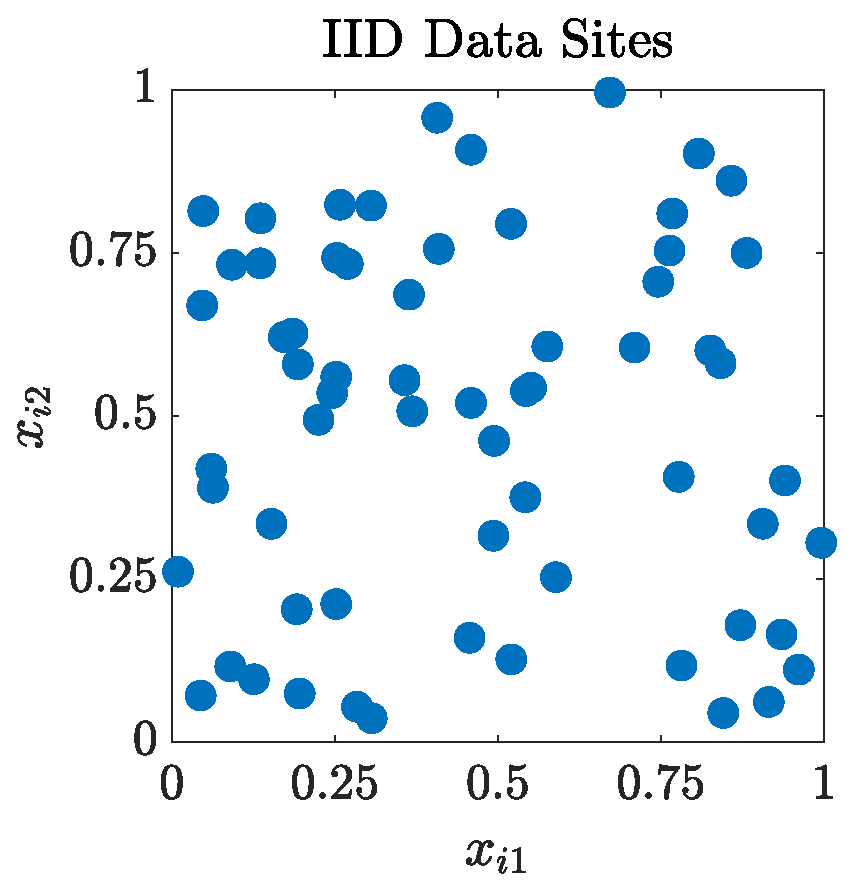
\includegraphics[width = 0.20\textwidth]{ProgramsImages/IIDPoints.eps} \ 
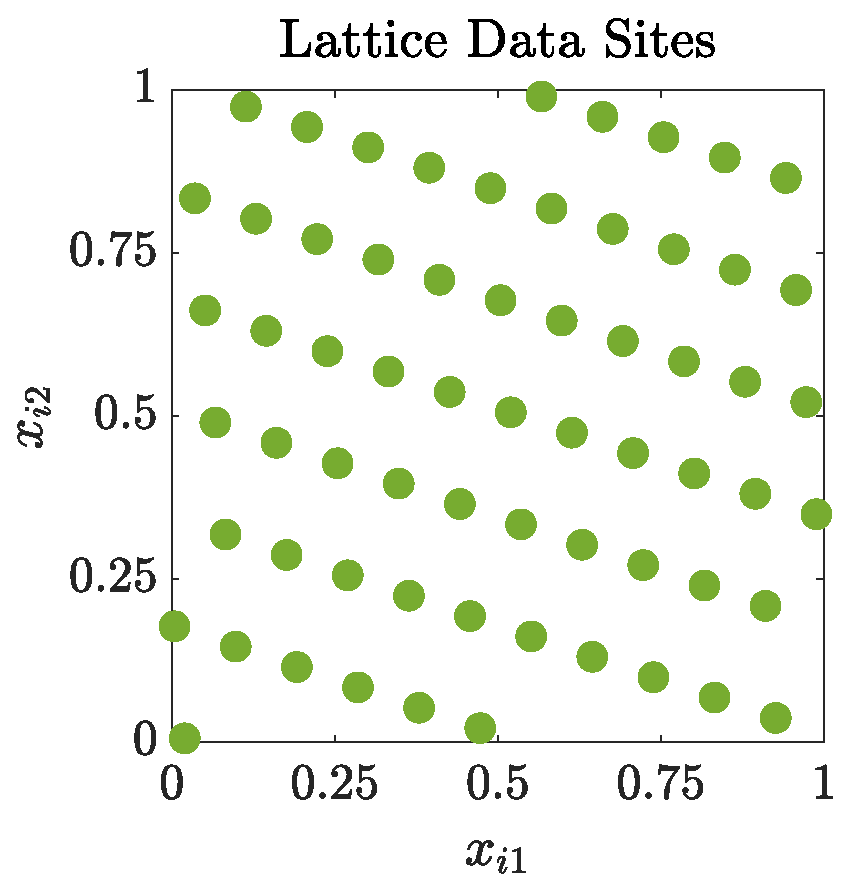
\includegraphics[width = 0.20\textwidth]{ProgramsImages/ShiftedLatticePoints.eps} \ 

\includegraphics[width = 0.20\textwidth]{ProgramsImages/ChebLatticePoints.eps} 
\caption{Uniform IID data sites contrasted with space filling designs mimicking the uniform  and arcsine distributions.
We will use low discrepancy space-filling sampling in our exploration stage.
\label{PtsFig}}
\end{wrapfigure}

We will compare the effectiveness of low discrepancy samples mimicking uniform and arcsine (Chebyshev) distributions.
The arcsine distribution pushes points towards the boundary of $\Omega$ so that there is sufficient data to interpolate $f$ there.  The advantage of doing so may depend on the smoothness of $f$ \cite{HicLi12a}.

Another approach for a space-filling exploratory design is to pick a typical reproducing kernel, $K$, as introduced in Sect.\ \ref{sec:varmodel}, and sequentially choose points to minimize $K(\bx,\bx) - \bk^T(\bx) \mK^{-1} \bk(\bx)$, where the Gram matrix $\mK$ is defined below in $\eqref{appxExOne}$. 

In some applications one may be able to obtain cheap data from certain sites.  There may be also prior data collected from earlier experiments.  Our initial exploration stage will include this data as well.


This exploratory set of $n_0$  sites does not depend on $f$ or the QOIs.  It must be small enough to be economical, but large enough to detect important features of $f$ that influence $\QOI(f)$. The large scale simulation is run for each of these POI vectors to obtain $f(\bx_1), \ldots, f(\bx_{n_0})$, and then we begin the exploitation stage.

%%%%%%%%%%%%%%%%%%%%%%%%%%%%%%%%%%%%%%%%%%%%%%%%%%%%%%%%%%%%%%%%%%%%%%%%%%%%%%%%%%%
\subsection{The Exploitation Stage: Surrogate Model and Acquisition} \label{sec:SurrMod}
%%%%%%%%%%%%%%%%%%%%%%%%%%%%%%%%%%%%%%%%%%%%%%%%%%%%%%%%%%%%%%%%%%%%%%%%%%%%%%%%%%%

In the exploitation stage, we create surrogate models, $\SURR(n,\mX,\by)$ defined on $\Omega$ by combining an MLS model to capture the mean-field behavior of the response surface with a 
variation RKHS minimum norm interpolant or kriging Gaussian Process model to estimate the variation in the model. 
%%%%%%%%%%%%%%%%%%%%%%%%%%%%%%%%%%%%%%%%%%%%%%%%%%%%%%%%%%%%%%%%%%%%%%%%%%%%%%%%%%%
\subsubsection{The Trend Model via MLS} \label{sec:trend}
%%%%%%%%%%%%%%%%%%%%%%%%%%%%%%%%%%%%%%%%%%%%%%%%%%%%%%%%%%%%%%%%%%%%%%%%%%%%%%%%%%%
We define our trend model as the MLS approximant
\begin{equation} \label{eq:MLS}
\STREND(n,\mX,\by)(\bx) = f_{\LS,\bx}(\bx), \qquad \text{where } f_{\LS,\bx} = \argmin_{g \in \calp} \sum_{i=1}^n w_i(\bx)(y_i - g(\bx_i))^2,
\end{equation}
and $\calp$ is a finite dimensional vector space, e.g., low degree polynomials. The weights $w_i(\bx)$ decrease with distance $\norm[2]{\bx - \bx_i}$. We will initially use a Gaussian kernel weight, $w_i(\bx) = \me^{-\norm[2]{\bx - \bx_i}^2/\sigma(\bx)^2}$, where $\sigma(\bx)$ is the mean distance from the evaluation point, $\bx$, to a set of $K_n$ nearest neighbors. The number of nearest neighbors will be greater than $\dim(\calp)$.

Every time the MLS interpolant is evaluated, we solve a least squares system that weights the nearby points much more than the distant points. For the problems we are considering,
\begin{wrapfigure}{r}{0.5\textwidth}
\begin{center}
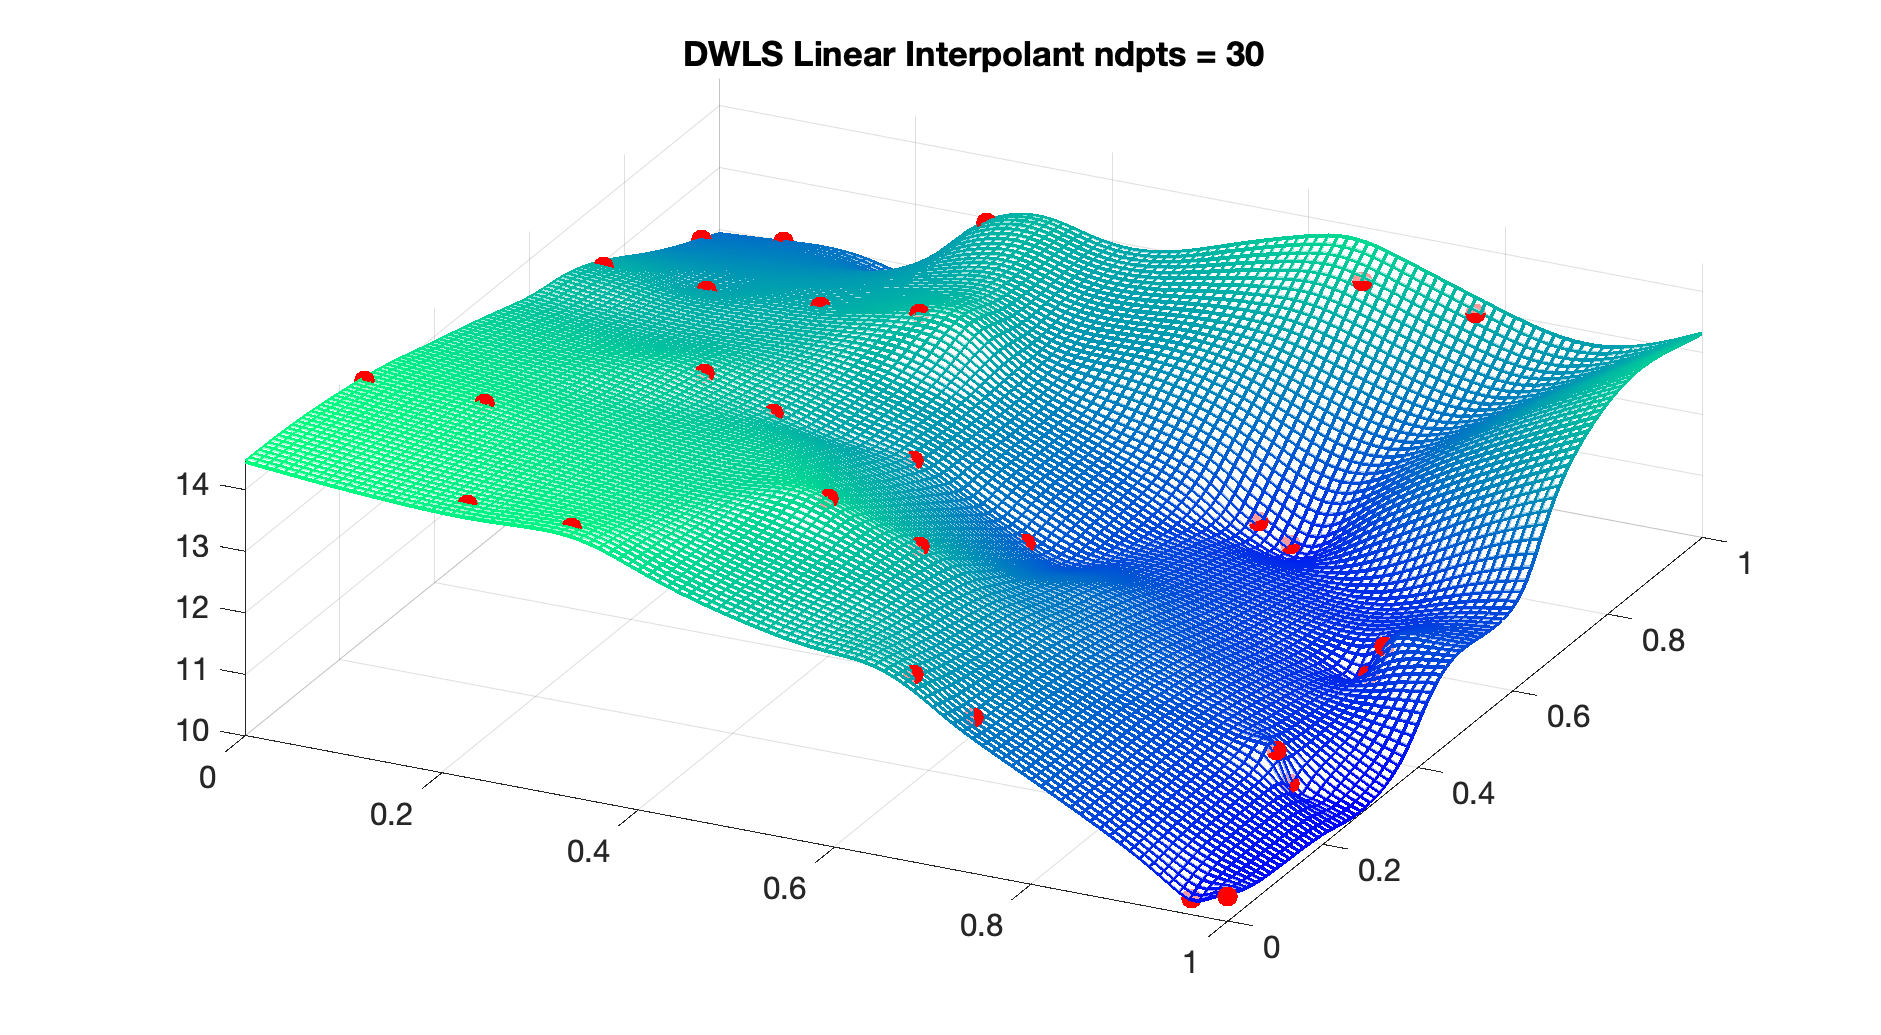
\includegraphics[width = 0.5\textwidth]{ProgramsImages/bigsurT.pdf}
\end{center}
\caption{The MLS quasi-interpolant with linear basis functions of scattered data {$\color{red}*$} of Big Sur sea bottom data \cite{franke1979critical}. The locally linear MLS trend model is able to fit very irregular surfaces.
\label{MLS}}
\end{wrapfigure}
this additional computation is minimal compared to the expense of obtaining the sample values. Note that the trend model exactly reproduces any $f \in \calp$.

If $\calp$ consists of all polynomials of total degree up to $k$, then $\dim(\calp)$ grows as ${k + d \choose k}$ and will far exceed $n$ for even modest $k$ and high $d$. 
We will typically choose $\calp$ to be quadratic polynomials for low dimensional problems $d<10$, and linear polynomials for high-dimensional problems. 
Global low-degree polynomial approximants are `stiff' and cannot bend to follow odd surfaces. The flexibility in MLS approximants using local low-degree polynomials is similar to the way splines fit data in one dimension. 
Figure \ref{MLS} illustrates the flexibility of an MLS with a local linear basis function fitting scattered data in two dimensions. 


%%%%%%%%%%%%%%%%%%%%%%%%%%%%%%%%%%%%%%%%%%%%%%%%%%%%%%%%%%%%%%%%%%%%%%%%%%%%%%%%%%%
\subsubsection{The Variation Model via RKHS/Kriging} \label{sec:varmodel}
%%%%%%%%%%%%%%%%%%%%%%%%%%%%%%%%%%%%%%%%%%%%%%%%%%%%%%%%%%%%%%%%%%%%%%%%%%%%%%%%%%%
The trend model, $\STREND(n,\mX,\by)$, is a quasi-interpolant because it does not exactly fit the data. Having modeled the general trend of the output map $f$, we now model its variation, $f_{\VAR} = f - \STREND(n,\mX,\by)$, using a minimum norm RKHS interpolant. Suppose that $f_{\VAR}$, belongs to an RKHS $\calf$. A commonly used reproducing kernel is the squared exponential (or Gaussian) kernel:
\begin{equation} \label{eq:GaussKer}
K(\bt,\bx) =  \exp(-\norm[2]{\btheta \odot (\bt-\bx)}^2),
\end{equation}
where $\odot$ denotes the term-by-term (Hadamard) product, and $\btheta \in (0, \infty)^d$ is a parameter to be set or inferred. See \cite{Buh00, Fas07a, FasMcC15a, ForFly15a, ForEtal09, SchWen06a, Wen05a} for an explanation of function approximation in RKHSs. The minimum norm interpolant of $f_{\VAR}$ in this $\calf$ using the residual data, $
\by_{\VAR} = \by - \by_{\TREND}$, where $\by_{\TREND} = \bigl(\STREND(n,\mX,\by)(\bx_i) \bigr)_{i=1}^n$,
is the surrogate variation model
\begin{equation} \label{appxExOne}
\SVAR(n,\mX,\by_{\VAR}) = \sum_{i=1}^n c_i K(\cdot, \bx_i), \quad \text{where } \bc = \mK^{-1} \by_{\VAR}, \quad \mK = \mK(\mX) = \bigl( K(\bx_i,\bx_j) \bigr)_{i,j=1}^n, 
\end{equation}
This has a known pointwise error bound of
\begin{align}
\label{eq:RKHSErrBd}
\abs{f(\bx) - \SVAR(n,\mX,\by_{\VAR})(\bx)} & \le \sqrt{K(\bx,\bx) - \bk^T(\bx) \mK^{-1} \bk(\bx)} \, \norm[\calf]{f_{\VAR} - \SVAR(n,\mX,\by_{\VAR})} \\
\nonumber
& \le \sqrt{K(\bx,\bx) - \bk^T(\bx) \mK^{-1} \bk(\bx)} \, \norm[\calf]{f_{\VAR}} \qquad \forall f_{\VAR} \in \calf, \ \bx \in \Omega, \\
\nonumber
& \qquad \qquad \text{where } \bk(\bx) = \bigl(K(\bx,\bx_i) \bigr)_{i=1}^n.
\end{align}
The choice of the kernel and the parameter $\btheta$ is addressed in Sect.\ \ref{sec:kerinferdata}.

The deterministic framework using RKHSs for $f_{\VAR}$ has a parallel Bayesian interpretation or probabilistic numerics promoted by Diaconis \cite{Dia88a} and other scientists \cite{BriEtal18a, OHa91a, OwhEtal19a, RasWil06a, Rit00a}. It assumes that $f_{\VAR}$ is an instance of $\GP(0,K)$, a Gaussian process with mean zero and covariance kernel, $K$. In this case the posterior mean of $f_{\VAR}(x)$ given the data $(\mX,\by)$ is called a kriging model and has the same expression as $\SVAR(n,\mX,\by)$ as in \eqref{appxExOne}, and the width of the pointwise credible interval for the surrogate variation model is the same as $\SVARERR(n,\mX,\by)$ in \eqref{eq:DataErrBd}, with $A(\mX)$ determined by empirical Bayes and dependent only on $n$. We will adopt both deterministic and Bayesian approachs, depending on which better suits our needs.



%%%%%%%%%%%%%%%%%%%%%%%%%%%%%%%%%%%%%%%%%%%%%%%%%%%%%%%%%%%%%%%%%%%%%%%%%%%%%%%%%%%
\subsubsection{Acquisition via the Surrogate Model} \label{sec:acquire}
%%%%%%%%%%%%%%%%%%%%%%%%%%%%%%%%%%%%%%%%%%%%%%%%%%%%%%%%%%%%%%%%%%%%%%%%%%%%%%%%%%%

Along with the surrogate model, $\SURR(n,\mX,\by)$, we must construct a data-based pointwise error bound or measure of its uncertainty, $\SURRERR(n,\mX,\by)$ (see \eqref{eq:surrUncert}).  That requires translating the error bound in \eqref{eq:RKHSErrBd} into a quantity that does not require a priori the knowledge of $\norm[\calf]{f_{\VAR} - \SVAR(n,\mX,\by_{\VAR})}$.  Our approach is discussed in Sects.\ \ref{sec:BayesianBootUncertainty} and \ref{sec:uncertVar}.

Given the surrogate model and its uncertainty, we may then define the acquisition functions for function and approximation respectively:
\begin{subequations} \label{eq:QOIval}
\begin{align}
\label{eq:idval}
\IDVAL(\bx,n,\mX,\by) &= \SURRERR(n,\mX,\by)(\bx), \\
\label{eq:minval}
\MINVAL(\bx,n,\mX,\by) &= \APPMIN(n,\mX,\by) - [\SURR(n,\mX,\by)(\bx) - \SURRERR(n,\mX,\by)(\bx)].
\end{align}
\end{subequations}
The next data site, $\bx_{n+1}$ maximizes the acquisition function (see \eqref{eq:nextsample}). For function approximation we sample next where the surrogate model uncertainty is greatest. For optimization we sample next where the output might be smallest.

To maximize the acquisition functions, we first evaluate them over a relatively dense set, $\ct = \{\bt_1, \ldots, \bt_N\}$ with $N \gg n$. We may then choose $\bx_{n+1} = \argmax_{\bt \in \ct} \VAL(\bt, n,\mX,\by)$.  Alternatively, we may use the elements of $\ct $ that give the largest values of $\VAL(\cdot, n,\mX,\by)$ as starting values for a numerical optimization algorithm to find the maximum of the acquisition function. We will consider both of these approaches. 

The acquisition functions are related to the error bounds that we expect to derive for our algorithms:
\begin{subequations} \label{eq:QOIerr}
\begin{align}
\label{eq:iderr}
\bignorm[\infty]{f - \APPID(n,\mX,\by)} &\le \norm[\infty]{\SURRERR(n,\mX,\by)} =: \IDERR(n,\mX,\by), \\
\label{eq:minerr}
\bigabs{\MIN(f) - \APPMIN(n,\mX,\by)} & \le \max_{\bx \in \Omega} \Bigl\{ \APPMIN(n,\mX,\by) - [\SURR(n,\mX,\by)(\bx) - \SURRERR(n,\mX,\by)](\bx) \Bigr\} \\
\nonumber
& =: \MINERR(n,\mX,\by).
\end{align}
\end{subequations}
These error bounds should be valid for $\calc$, precisely defined candidate sets of well-behaved simulation output maps, $f$. The identification of these $\calc$ is part of our research. Hints appear in Sect.\ \ref{sec:uncertVar}. 

\subsection{Algorithmic Framework} \label{sec:algo}
The algorithm that we will develop and analyze will have the following form.

\begin{algorithm}[H]
	\caption*{Adaptive Algorithm to Approximate $\QOI(f)$ \label{alg:algframe}}
	\begin{algorithmic}
		\PARAM a candidate set (cone) of input functions, $\cc$; the set of local basis functions for MLS approximation of the trend, $\cP$; the MLS weight function; the parameterized reproducing kernel  $K_{\btheta}$; an initial sample size, $n_0$
		\INPUT a black-box function, $f \in \cc$; an absolute error tolerance, $\varepsilon>0$
		
		\Ensure Error criterion $\bignorm[\infty]{\QOI(f) - \APP(n,\mX,\by)} \le \varepsilon$  for $f \in \cc$
		
		\State Let $n \leftarrow n_0$
		
		\State Construct data sites $\mX$ according to Sect.\ref{sec:Explore}  \Comment{ \textbf{Explore}}
		
		\Repeat \Comment{ \textbf{Exploit}}
		
		\State Update $\by = f(\mX)$
		
		\State Compute the  trend, $\STREND(n,\mX,\by)$, by moving least squares according to Sects.\ \ref{sec:trend} and \ref{sec:ourtrend}
		
		\State Compute the variation, $\SVAR(n,\mX,\by)$, as a minimum norm RKHS interpolant according to Sects.\ \ref{sec:varmodel}, \ref{sec:uncertVar} and \ref{sec:kerinferdata}
		
		\State Compute the  uncertainty in the surrogate model, $\SURRERR(n,\mX,\by)$, according to Sects.\ \ref{sec:uncertVar} and \ref{sec:BayesianBootUncertainty}
		
		\State Construct error bound $\ERR(n,\mX,\by)$ for approximation $\APP(n,\mX,\by)$ via \eqref{eq:QOIerr} using the surrogate model, $\SURR(n,\mX,\by) = \STREND(n,\mX,\by) + \SVAR(n,\mX,\by)$, and its uncertainty, $\SURRERR(n,\mX,\by)$.
		
		\If{$\ERR(n,\mX,\by) \le \varepsilon$}
		
		\RETURN $\APP(n,\mX,\by)$ as computed in \eqref{eq:QOIhat}
		
		\EndIf
				
		\State Choose the next data site $\bx_{n+1}$ according to \eqref{eq:nextsample}, where the acquisition function, $\VAL(\mX,\by)$, is defined in \eqref{eq:QOIval}
		
		\State Let $n \leftarrow n + 1$

		\Until $n > n_{\max}$
				
	\end{algorithmic}
\end{algorithm}

Some of these ideas have been described earlier in this section.  The more novel ones are described in the next section.

\subsection{Alternative Approaches}
Before fleshing out the algorithm above, we review some alternative  approaches.

%%%%%%%%%%%%%%%%%%%%%%%%%%%%%%%%%%%%%%%%%%%%%%%%%%%%%%%%%%%%%%%%%%%%%%%%%%%%%%%%%%%%
\subsubsection{Existing Adaptive Sampling Schemes and Their Shortcomings} \label{sec:shortExist}
%%%%%%%%%%%%%%%%%%%%%%%%%%%%%%%%%%%%%%%%%%%%%%%%%%%%%%%%%%%%%%%%%%%%%%%%%%%%%%%%%%%

We summarize the existing literature on adaptive sampling \cite{aute2013cross,burnaev2015adaptive,fu2017adaptive,gramacy2008adaptive,jin2002sequential,kleijnen2004application}. A number of popular adaptive design criteria are constructed based on an acquisition function that does not depend on the simulation output data, but only on the data sites, i.e., $\VAL(n,\mX,\by) = \VAL(n,\mX)$. Such adaptive designs fill in holes in the existing design according to particular criteria, including those below. 
\begin{description}
	\item[Discrepancy] This measures the difference between the empirical distribution of the design and the target (uniform, arcsine, etc.) distribution \cite{FangEtal19a}. Examples of low discrepancy designs are given in Fig.\ \ref{PtsFig}. 
	\item[Covering radius or fill distance] This is the minimum radius needed for balls centered at each data site to cover the whole domain, $\Omega$. Minimax designs minimize this criterion.  These do not scale well to higher dimensions unless the distance measure is non-isotropic.
	\item[Minimium distance between data sites] Maximin designs maximize this criterion \cite{jin2002sequential}.  These also do not scale well to higher dimensions unless the distance measure is non-isotropic.
	\item[Entropy] Designs maximizing entropy seek to maximize the information when choosing the next data site \cite{jin2002sequential}. They also typically assume a known Gaussian process model.
\end{description}
Space-filling designs will be candidates for our exploration stage, but not our exploitation stage, because they do not take advantage of function data.  We will explore which ones work best for our test cases and application problems.

Orthogonal arrays and Latin hypercube sampling are further examples of space-filling designs, although they are not usually constructed sequentially. Grids do not fill space, are not sequential, and are not efficient in high dimensions.  Sparse grids \cite{BunGrie04a} are an improvement, but the number of points required can still be impractical in high dimensions.  
%Using this approach alone to fill the domain with samples is less efficient than the exploitation stage because it does not use the output data in a meaningful way. 

Some existing adaptive sampling methods use a jackknife and leave-one-out cross-validation adaptive sampling to measure the variation in predictions based on leaving out one observation at a time \cite{aute2013cross,jin2002sequential, kleijnen2004application}. However, these approaches often tend to pick the next data site close to an existing one \cite{jin2002sequential}, which is wasteful. A fix has been proposed to include a penalty that discourages choosing the next data site close to an existing one \cite{aute2013cross,jin2002sequential}.

\subsubsection{Alternative Function Approximation Algorithms and Their Shortcomings} \label{sec:shortAlgo}

There are some approaches to multivariate approximation that we are unlikely to pursue.  
\begin{description}
	\item[Multivariate polynomials] They are inflexible because they limit the approximation to a finite dimensional space, and they must be of low degree in high dimensions to avoid the curse of dimensionality.
	\item[Smolyak Algorithms \cite{BunGrie04a}] Because they are based on sparse grids have the weaknesses mentioned above for sparse grids.  Moreover, any algorithm based on a grid will have challenges if we want to rotate the coordinate system to identify a low dimensional structure.
	\item[Continuous Tensor Trains \cite{GorKarMar19a}] Chebfun \cite{DriHalTre14a} employs this method for low dimensional multivariate function approximation, but it does not scale well to high dimensions.
\end{description}


%%%%%%%%%%%%%%%%%%%%%%%%%%%%%%%%%%%%%%%%%%%%%%%%%%%%%%%%%%%%%%%%%%%%%%%%%%%%%%%%%%%
\section{Intellectual Merit of the Proposed Research} \label{sec:Proposed}
%%%%%%%%%%%%%%%%%%%%%%%%%%%%%%%%%%%%%%%%%%%%%%%%%%%%%%%%%%%%%%%%%%%%%%%%%%%%%%%%%%%


%%%%%%%%%%%%%%%%%%%%%%%%%%%%%%%%%%%%%%%%%%%%%%%%%%%%%%%%%%%%%%%%%%%%%%%%%%%%%%%%%%%
\subsection{Surrogate Trend Models} \label{sec:ourtrend}
%%%%%%%%%%%%%%%%%%%%%%%%%%%%%%%%%%%%%%%%%%%%%%%%%%%%%%%%%%%%%%%%%%%%%%%%%%%%%%%%%%%
Global parametric surrogate models can capture the trend of a multivariate response surface only if the data are fit well by the parametric model over all the domain. For example, in one-dimensional problems, global low-degree polynomials can capture simple trends in the data, but fail to accurately represent nonpolynomial shapes, such as Gaussians or step functions. Piecewise polynomial interpolants, such as tensor splines, can effectively represent these surfaces, but don't generalize easily to very high dimensions with scattered data. 

The MLS quasi-interpolants are an effective alternative to piecewise polynomials in high dimensions. The MLS uses local low-degree polynomials to capture global nonpolynomial behavior. The additional computational cost to solve for the local MLS coefficients is small compared to the cost of generating new function data. 

One of the challenges in MLS is to identify a robust methodology for picking the appropriate length scale, $\sigma(\bx)$, for the MLS kernel. Our current approach is to define this length scale as the mean distance to the nearest $K_n$ neighbors of $\bx$, where $K_n$ is greater than $\dim(\calp)$, the dimension of the space of local approximants.
This heuristic approach usually identifies a good balance between the relative weights of the nearby and distant points so that the Moore Penrose matrix for the least squares problem is well-conditioned. If the least squares problem is ill-conditioned, then the length scale is increased. \emph{We propose to analyze this heuristic approach and identify a procedure, along the lines of the adaptive Armijo rule in numerical optimization \cite{kelley1999iterative}, to select the local length scale based on a more mathematical foundation.}  We will also investigate the local scaling approach of \cite{ZelPer05a}.

Another shortcoming of the existing MLS quasi-interpolants is that they treat every coordinate direction the same. 
\emph{We will extend the MLS to use the full covariance matrix in the multivariate Gaussian kernel based on the relative variation in underlying active dimensional analysis}. We will describe some of these ideas in section \ref{sec:kerinferdata}. 




\subsection{Uncertainty in the Variation Model} \label{sec:uncertVar}
To construct a data-driven error bound for the variation, $f_{\VAR}$, in terms of the theoretical error bound in \eqref{eq:RKHSErrBd}, we must bound the norm of $f_{\VAR}$ in terms of function data.  To do this we introduce a cone $\calc$ of candidate functions whose norms are approximated modestly well by the norms of their surrogates: 
\begin{align} \label{RKHScone}
	\calc &:= \Bigl\{f_{\VAR} \in \calf : \norm[\calf]{f_{\VAR} - \SVAR(n,\mX,\by_{\VAR})} \le A(\mX) \bignorm[\calf]{\SVAR(n,\mX,\by_{\VAR})} \Bigr \} \\
	\nonumber
	& = \Bigl\{f_{\VAR} \in \calf : \norm[\calf]{f_{\VAR}}^2 \le (1 + A^2(\mX)) \bignorm[\calf]{\SVAR(n,\mX,\by_{\VAR})}^2 \Bigr \},
\end{align}
where $A(\mX)$ is positive and fixed in advance. This $\calc$ is a cone because if $f_{\VAR} \in \calc$, then $c f_{\VAR} \in \calc$ for any real $c$. The intuition in defining this cone is: \emph{what you have not seen is not much worse than what you can see}. All adaptive algorithms are based on this philosophy. The definition of the cone in \eqref{RKHScone} is a way of formalizing this key idea. Noting that $\bignorm[\calf]{\SVAR(n,\mX,\by_{\VAR})} = \sqrt{\by_{\VAR} \mK^{-1} \by_{\VAR}}$ error bound \eqref{eq:RKHSErrBd} then implies an error bound that can be computed solely based on the output data: 
\begin{subequations} \label{eq:DataErrBd}
	\begin{gather}
		\abs{f_{\VAR}(\bx) - \SVAR(n,\mX,\by_{\VAR})(\bx)} \le \SVARERR(n,\mX,\by_{\VAR})(\bx) \qquad \forall f \in \calc, \\
		\label{eq:DataErrBda} 
		\text{where } \SVARERR(n,\mX,\by_{\VAR})(\bx) : = A(\mX) \sqrt{[K(\bx,\bx) - \bk^T(\bx) \mK^{-1} \bk(\bx)] \, [\by_{\VAR}^T \mK^{-1} \by_{\VAR}] }.
	\end{gather}
\end{subequations}
This idea of data-driven error bounds for numerical problems has been used by \FH, \YD, and their collaborators in \cite{HicEtal14a, HicEtal14b, HicJim16a, JimHic16a, HicEtal17a, ChoEtal17a}.



%%%%%%%%%%%%%%%%%%%%%%%%%%%%%%%%%%%%%%%%%%%%%%%%%%%%%%%%%%%%%%%%%%%%%%%%%%%%%%%%%%%
\subsection{Inferred Kernels for Surrogate Variation Models} \label{sec:kerinferdata}
%%%%%%%%%%%%%%%%%%%%%%%%%%%%%%%%%%%%%%%%%%%%%%%%%%%%%%%%%%%%%%%%%%%%%%%%%%%%%%%%%%%

While  \eqref{eq:DataErrBd}  provides a data-driven error bound for the surrogate variation, there still remains the question of which kernel to choose.  For example, the squared exponential kernel in \eqref{eq:GaussKer} has the parameter $\btheta$ that must be specified.

We will experiment with the empirical Bayes perspective, which leads to the following choice \cite{Hic17a}: 
\begin{equation} \label{eq:thetEB}
	\btheta_{\textup{EB}} = \argmin_\btheta \left[\frac 1n \log \bigl( \det(\mK_\btheta) \bigr) + \log \bigl ( \by^T \mK_\btheta^{-1} \by \bigr)\right].
\end{equation}
This criterion also has a purely geometric interpretation.  Cross-validation is another possibility.  

As proof of concept we consider the function
\begin{equation} \label{eq:cos_sum}
	f_V(\bx) =  \cos( \alpha_1 x_1 + \cdots + \alpha_d x_d), \quad \bx \in [0,1]^d, \qquad \alpha_\ell = 2^{-\pi_d(\ell)}, \ell = 1, \ldots, d,
\end{equation}
where $\pi_d$ is a permutation of the integers $1, \ldots, d$.  The reason that we choose some coordinates as less important than others is to provide a low essential dimension.  The reason for the permutation of coordinate indices is to illustrate how our process does not require a priori knowledge of the relative importance of the coordinates.

Table  \ref{tab:cos_sum} is the output of a stripped-down version of our algorithm in Sect.\ \ref{sec:algo} without the trend applied to \eqref{eq:cos_sum} with $d=12$. We take $\SVARERR(n,\mX,\by_{\VAR})$ to be the pointwise uncertainty in the surrogate model.  For $A(\mX)$ we use
\begin{equation*} \label{eq:an}
	A(\mX): = \begin{cases} \displaystyle
		\frac{0.2}{0.2 - B(\mX)}, & B(\mX) < 0.2, \\
		\infty, & B(\mX) \ge 0.2, 
	\end{cases}
\qquad 
B(\mX) : = \sqrt{K(\bx,\bx) - \bk^T(\bx) \mK^{-1} \bk(\bx)}.
\end{equation*}
As the design improves, the inflation factor, $A(\mX)$ becomes smaller. 
The exploratory design is $n_0 = 10$ uniform lattice points.  For performing the sup-norm calculations, we use $\ct$ consisting of $2^{16}$ uniform lattice points on 

The adaptive algorithm successfully computes the approximation, $\APPID(n,\mX,\by)$, which satisfies the sequence of error tolerances via adaptive sampling and an data-driven error bound, $\ERR(n,\mX,\by) = \norm[\infty]{\SVARERR(n,\mX,\by_{\VAR})}$.  Moreover, the pointwise data-driven error bound in  \eqref{eq:DataErrBd} is successful $100\%$ of the points in $\ct$.


\begin{table}
	\caption{Adaptive algorithm successfully applied to \eqref{eq:cos_sum} for different error tolerances.} \label{tab:cos_sum}

\[ 
\begin{array}{rccccccc} 
\hline 
	\text{Coordinate}, \ell & 10 & 1  & 7 & 5 & 9 & 8 \\
	\alpha_\ell & 5.0\text{E}{-}1 & 2.5\text{E}{-}1 & 1.3\text{E}{-}1  & 6.3\text{E}{-}2 &3.1\text{E}{-}2& 1.6\text{E}{-}2 \\
	\theta_\ell & 2.2\text{E}{-}1  & 1.2\text{E}{-}1 & 6.3\text{E}{-}2 & 3.1\text{E}{-}2 & 1.4\text{E}{-}2& 9.2\text{E}{-}3, \\
	\hline
	\text{Coordinate},\ell & 12 & 4 & 6 & 3 & 2 & 11 \\
	\alpha_\ell & 7.8\text{E}{-}3 & 3.9\text{E}{-}3 & 2.0\text{E}{-}3 & 9.8\text{E}{-}4 & 4.9\text{E}{-}4 & 2.4\text{E}{-}4\\
	\theta_\ell & 4.5\text{E}{-}3 & 2.1\text{E}{-}3&  1.2\text{E}{-}3 & 8.9\text{E}{-}4& 5.4\text{E}{-}8& 7.1\text{E}{-}5\\
	\hline
	n &  18 &  22 &  29 &  36 &  48 &  65 &  87 \\ \hline 
	\varepsilon & 1.0\text{E}{-}1 & 5.0\text{E}{-}2 & 2.0\text{E}{-}2 & 1.0\text{E}{-}2 & 5.0\text{E}{-}3 & 2.0\text{E}{-}3 & 1.0\text{E}{-}3 \\ \hline 
	\norm[\infty]{\SVARERR(n,\mX,\by_{\VAR})}  & 8.2\text{E}{-}2 & 4.3\text{E}{-}2 & 2.0\text{E}{-}2 & 9.4\text{E}{-}3 & 4.7\text{E}{-}3 & 2.0\text{E}{-}3 & 1.0\text{E}{-}3 \\ \hline 
	\rule[3ex]{0pt}{0pt} \bignorm[\infty]{f - \APPID(n,\mX,\by)}  & 2.5\text{E}{-}2 & 1.0\text{E}{-}2 & 6.8\text{E}{-}3 & 4.4\text{E}{-}3 & 1.1\text{E}{-}3 & 1.8\text{E}{-}3 & 4.5\text{E}{-}4 \\ \hline 
	\text{Ptwise Error Bound} & 100\% & 100\% & 100\% & 100\% & 100\% & 100\% & 100\% 
\end{array} 
\]
\end{table}

Choosing different $\theta_\ell$ in the definition of the reproducing kernel has been studied by \FH and his collaborators \cite{FasHicWoz12a, FasHicWoz12b}.  It is an example of \emph{coordinate weights}, which arise in the tractability literature for continuous numerical problems (see \cite{DicEtal14a,NovWoz08a, NovWoz10a, NovWoz12a} and the references therein).  Small $\theta_\ell$ means that the $x_\ell$ does not influence the function $f$ much.  If many of the $\theta_\ell$ are small then the effective dimension of the function is much smaller than the nominal dimension, $d$, and the problem is tractable.

An extension of this idea of coordinate weights is to rotate the original POIs to obtain a new coordinate system whose variables are arranged in order of importance. This approach is described as identifying \emph{active subspaces} and is championed in \cite{constantine2015active}. We may incorporate this idea by generalizing \eqref{eq:GaussKer} to become 
\begin{equation} \label{eq:multisqExpD}
	K(\bt,\bx) = \exp(-\norm[2]{\mD \mR(\bt-\bx)}), 
\end{equation}
where $\mD$ is a diagonal matrix containing the coordinate weights, and $\mR$ is rotation matrix composed of $d-1$ Givens rotations.  Thus, the selection of an optimal $\mD$ and $\mR$ via \eqref{eq:thetEB} would involve $2d-1$  elements of $\btheta$.  We will \emph{explore whether active subspaces can help us avoid the curse of dimensionality}.

The Gaussian kernel, may be a good choice, but there is a whole family of Mat\'ern kernels of order $\nu >0$ of which the Gaussian kernel is the $\nu \to \infty$ limit.  We will explore including $\nu$ as an element of $\btheta$ to be optimized.  We may also investigate other parameterized families of reproducing kernels.


\iffalse
%%%%%%%%%%%%%%%%%%%%%%%%%%%%%%%%%%%%%%%%%%%%%%%%%%%%%%%%%%%%%%%%%%%%%%%%%%%%%%%%%%%
\Upara{Nonhomogeneous Distance for MLS}
%%%%%%%%%%%%%%%%%%%%%%%%%%%%%%%%%%%%%%%%%%%%%%%%%%%%%%%%%%%%%%%%%%%%%%%%%%%%%%%%%%%
For the MLS algorithm used to construct the surrogate trend, $\STREND$, the weight assigned to the $i^{\text{th}}$ data is traditionally defined in terms of the Euclidean distance to that data site from to the location being approximated, i.e., $\norm[2]{\bx - \bx_i}$. To avoid the curse of dimensionality, we may \emph{employ some non-isotropic concept of distance} involving coordinate weights or identification of active subspaces.  For example, we may replace $\norm[2]{\bx - \bx_i}$ by $\norm[2]{\mD(\bx-\bx_i)}$ or $\norm[2]{\mD \mR(\bx - \bx_i)}$.  If the MLS basis set $\calp$, is comprised of linear polynomials, then the rescaling and rotating of the coordinates leaves this set unchanged in terms of the new variables $\bx' =  \mD \mR \bx$.
\fi

%%%%%%%%%%%%%%%%%%%%%%%%%%%%%%%%%%%%%%%%%%%%%%%%%%%%%%%%%%%%%%%%%%%%%%%%%%%%%%%%%%%
\subsection{Bayesian Bootstrapping to Determine Surrogate Trend Model Uncertainty} \label{sec:BayesianBootUncertainty}
%%%%%%%%%%%%%%%%%%%%%%%%%%%%%%%%%%%%%%%%%%%%%%%%%%%%%%%%%%%%%%%%%%%%%%%%%%%%%%%%%%%
The uncertainty in our surrogate variation models, $\SVARERR(n,\mX,\by)$, could serve as our surrogate model uncertainty. However, given the small number of data used to construct our models and the relatively large number of POIs involved, we propose to overlay another measure of uncertainty on top for the sake of robustness. 

In classical bootstrapping, new sets of samples are generated by randomly selecting the existing samples, with replacement. 
In small sample situations, removing even a few samples from the least squares fit can create significant variations in the trend model. In the weighted Bayesian bootstrap algorithm, all of the samples are used for each trend model, and the $i^{\text{th}}$ sample is randomly weighted by the factor $v_i \in [0,1]$. By using all the samples, the weighted Bayesian bootstrap method provides a more robust estimate for uncertainty quantification in small samples than the classical bootstrap method \cite{rubin1981bayesian, efron1986bootstrap, efron2016computer}. 

In our weighted Bayesian bootstrap algorithm, we generate an ensemble of $B$ trend models by extending \eqref{eq:MLS}:
\begin{equation}
	\STREND^b(n,\mX,\by)(\bx) = f^b_{\LS,\bx}(\bx), \qquad \text{where } f^b_{\LS,\bx} = \argmin_{g \in \calp} \sum_{i=1}^n v_i^b w_i(\bx)(y_i - g(\bx_i))^2,
\end{equation}
where as in Sect.\ \ref{sec:trend}, the $w_i$ are the MLS weight functions, and now $\bv^b$ is an $n$-vector uniformly distributed over the unit simplex, $\cals^n : = \{\bv \in [0,1]^n : v_1 + \cdots + v_n = 1\}$. We then define the bootstrap trend data as $\by^b_{\TREND} = \bigl(\STREND^b(n,\mX,\by)(\bx_i) \bigr)_{i=1}^n$. 

For each trend model, $\STREND^b(n,\mX,\by)$, we construct the an associated variation model, $\SVAR^b(n,\mX,\by - \by^b_{\TREND})$ and its uncertainty, $\SVARERR^b(n,\mX,\by - \by^b_{\TREND})$. These lead to our final surrogate model and its uncertainty.
The surrogate model for each Bayesian bootstrap model can be expressed as 
\begin{equation*}
	\SURR^b(n,\mX,\by) = \STREND^b(n,\mX,\by) + \SVAR^b(n,\mX,\by - \by^b_{\TREND}).
\end{equation*}
These can be averaged to define the mean surrogate model
\begin{equation} \label{eq:SMBoot}
	\SURR(n,\mX,\by) = \frac 1B \sum_{b=1}^B \SURR^b(n,\mX,\by), 
\end{equation}
and the surrogate uncertainty model is defined by the estimate
\begin{equation} \label{eq:SUBoot}
	\SURRERR(n,\mX,\by) = \sqrt{\frac{1}{B-1} \sum_{b=1}^B \Bigl\{ \bigl[ \SURR^b(n,\mX,\by) - \SURR(n,\mX,\by) \bigr]^2 + [\SVARERR^b(n,\mX,\by)]^2 \Bigr\} } .
\end{equation}
We are not certain if this simple estimate is the best measure of uncertainty. We will explore alternatives to identify possible better approaches to combine the ensemble of uncertainty estimates.


%%%%%%%%%%%%%%%%%%%%%%%%%%%%%%%%%%%%%%%%%%%%%%%%%%%%%%%%%%%%%%%%%%%%%%%%%%%%%%%%%%%
\subsection{Theoretical Aspects}
%%%%%%%%%%%%%%%%%%%%%%%%%%%%%%%%%%%%%%%%%%%%%%%%%%%%%%%%%%%%%%%%%%%%%%%%%%%%%%%%%%%

Up to now, we have outlined our algorithmic approach to adaptive sampling for function approximation and optimization. In Sects.\ \ref{sec:Applications} and \ref{sec:Software} we describe the applications we will use to demonstrate our algorithms and the software that we will produce.

We will also \emph{attempt to provide theoretical justification for our algorithms}. This involves identifying sets of output maps, $\calc$, for which our algorithms have guaranteed data-driven error bound. Because the identity map is homogeneous, i.e., $\ID(cf) = c\ID(f)$ for all $c \in \reals$, our surrogate models, $\SURR$, and surrogate uncertainties, $\SURRERR$, are also constructed to be homogeneous. It then follows that the sets of functions, $\calc$, for which the error bounds \eqref{eq:surrUncert} are guaranteed, are \emph{cones}, i.e., $f \in \calc \implies cf \in \calc$.

The challenge in identifying the suitable cones, $\calc$, is that we do not want them to be algorithm dependent. Our adaptive algorithms and sampling schemes will be defined in terms of $\calc$, but the definitions of $\calc$ should not depend on our algorithms or sampling schemes. Otherwise, we could simply define $\calc$ as the cones for which our algorithms succeed. This would be true but unenlightening.

Our algorithms are comprised of several parts, and some of those parts have an underdeveloped theory. Moreover, we are not restricting ourselves to a pre-set Banach space of output maps. Instead, we are learning the correct norm for $f$ as we sample adaptively. E.g., adaptively inferring the reproducing kernel is equivalent to learning the norm of the Hilbert space. Rather than focus on asymptotic convergence rates, our theory will be pre-asymptotic and focus on obtaining reliable, accurate approximations with a small number of samples. Given our success in developing the theory for adaptive algorithms in Sect.\ \ref{previousmeritsubsec}, and given the theory that does exist for the RKHS/kriging part, we expect to be able to fill in the gaps, in spite of these challenges.


%%%%%%%%%%%%%%%%%%%%%%%%%%%%%%%%%%%%%%%%%%%%%%%%%%%%%%%%%%%%%%%%%%%%%%%%%%%%%%%%%%%
\subsection{Applications} \label{sec:Applications}
%%%%%%%%%%%%%%%%%%%%%%%%%%%%%%%%%%%%%%%%%%%%%%%%%%%%%%%%%%%%%%%%%%%%%%%%%%%%%%%%%%%
\iffalse 
Our adaptive sampling algorithms will create computationally efficient algorithms with applications to 
\renewcommand{\descriptionlabel}[1]{\hspace{\labelsep}\textit{#1}.}
\begin{description}
\item[Function approximation] We will create surrogate models, with uncertainty estimates, that represent the output well over the entire feasible range of POIs using a minimal number of samples. This model can be used for global sensitivity analysis and dynamic (interactive) visualization of the response surface. 
\item[Optimization] We will use our surrogate models to identify multiple local optima of the response function. The local minima can then be used to identify as starting locations for gradient descent algorithms.
\end{description}
\fi

We will collaborate with modeling teams and apply our methodologies to guide both deterministic and stochastic large-scale simulations of climate change models and stochastic network models to predict disease transmission. 


\Upara{Los Alamos Sea Ice Model}
Accurate climate predictions depend on understanding the role that sea ice plays and how the ice couples with the ocean and atmospheric models.
%About nine million square miles of sea ice float on top of the world‚Äö high-latitude seas and oceans. Sea ice helps keep polar regions cool. It is constantly in motion and constantly changing internally. It influences Earth‚Äö climate, wildlife, and people who must contend with it year-round. Sea ice makes navigation difficult, creating challenges for commercial shipping, mining and energy development, fishing, hunting, tourism, scientific research, military bases, and defense operations. 
We will collaborate with Elizabeth Hunke (Los Alamos National Laboratory) to apply our methodology to predicting the sea ice environment. Hunke is the principal developer of the Los Alamos sea ice model (CICE) \cite{hunke2017cice, hunke2010cice}. This model incorporates physical effects of the atmosphere and ocean on the ice and accounts for the physical feedback mechanisms between the sea ice and the full Earth climate system models. Each CICE simulation can take hours to run, even on the world's fastest computers.

%Under the influence of wind and ocean currents, the fresh ice moves on the ocean surface, and melts. The melting creates a layer of fresher water that disrupts the ocean convection and vertical motion. This effect could modify the global “conveyor belt” (Gulf Stream) of heat moving through the world’s oceans and disrupt the entire Earth's environment. 
Hunke and her colleagues have conducted 150 CICE model simulations, selected to space-filling in the 39-dimensional space of feasible parameters. Of these, only about 100 of the runs were successful, due to parameter induced instabilities. They then added 400 low discrepancy Sobol' samples in regions where the simulation was stable. In these preliminary studies, they confirmed that the standard approaches \cite{bengio2006curse, o2010oxford} were not practical for their 39-dimensional sample space. We will use our two-part surrogate model to identify the active parameters \cite{constantine2014active} and predict the response between the sample points. 
\emph{We will collaborate with Hunke to quantify the sensitivity of the model predictions for sea ice coverage with respect to the 39 model parameters.} We will then identify the parameters where the next runs are predicted to most reduce the uncertainty in the surrogate model.
\Upara{Volcanic Impact on North Atlantic Oscillation}
Large volcanic eruptions inject massive amounts of SO${}_2$ into the upper atmosphere, where it is converted into sulfate aerosols. These aerosols reflect short-wave radiation and cause changes in the surface and sea surface temperatures, upper atmospheric winds, and global precipitation patterns \cite{zanchettin2013background, legrande2015volcanic,zanchettin2016model}. 
These large perturbations can lead to major changes in global climate patterns.

We will collaborate with Kostas Tsigaridis and Allegra LeGrande to help guide large-scale simulations using the Goddard Institute for Space Studies (GISS) large-scale climate model E2.1-R. \emph{Our goal will be to identify which new simulations will provide the most useful information to better understand the impact of volcanic eruptions on the climate.} MH is mentoring Helen Weierbach's undergraduate honor's thesis at Tulane using our surrogate model for some preliminary studies. Last summer, she worked at GISS with Tsigaridis and LeGrande as an undergraduate research intern. Weierbach will be collaborating with us to quantify the sensitivity of model predictions to the initial state of the North Atlantic Oscillation. 
%Other quantities of interest include the geopotential heights and upper atmosphere wind anomalies and sea level pressure in the North Atlantic basin. 

\begin{wrapfigure}{r}{0.3\textwidth}
\begin{center}
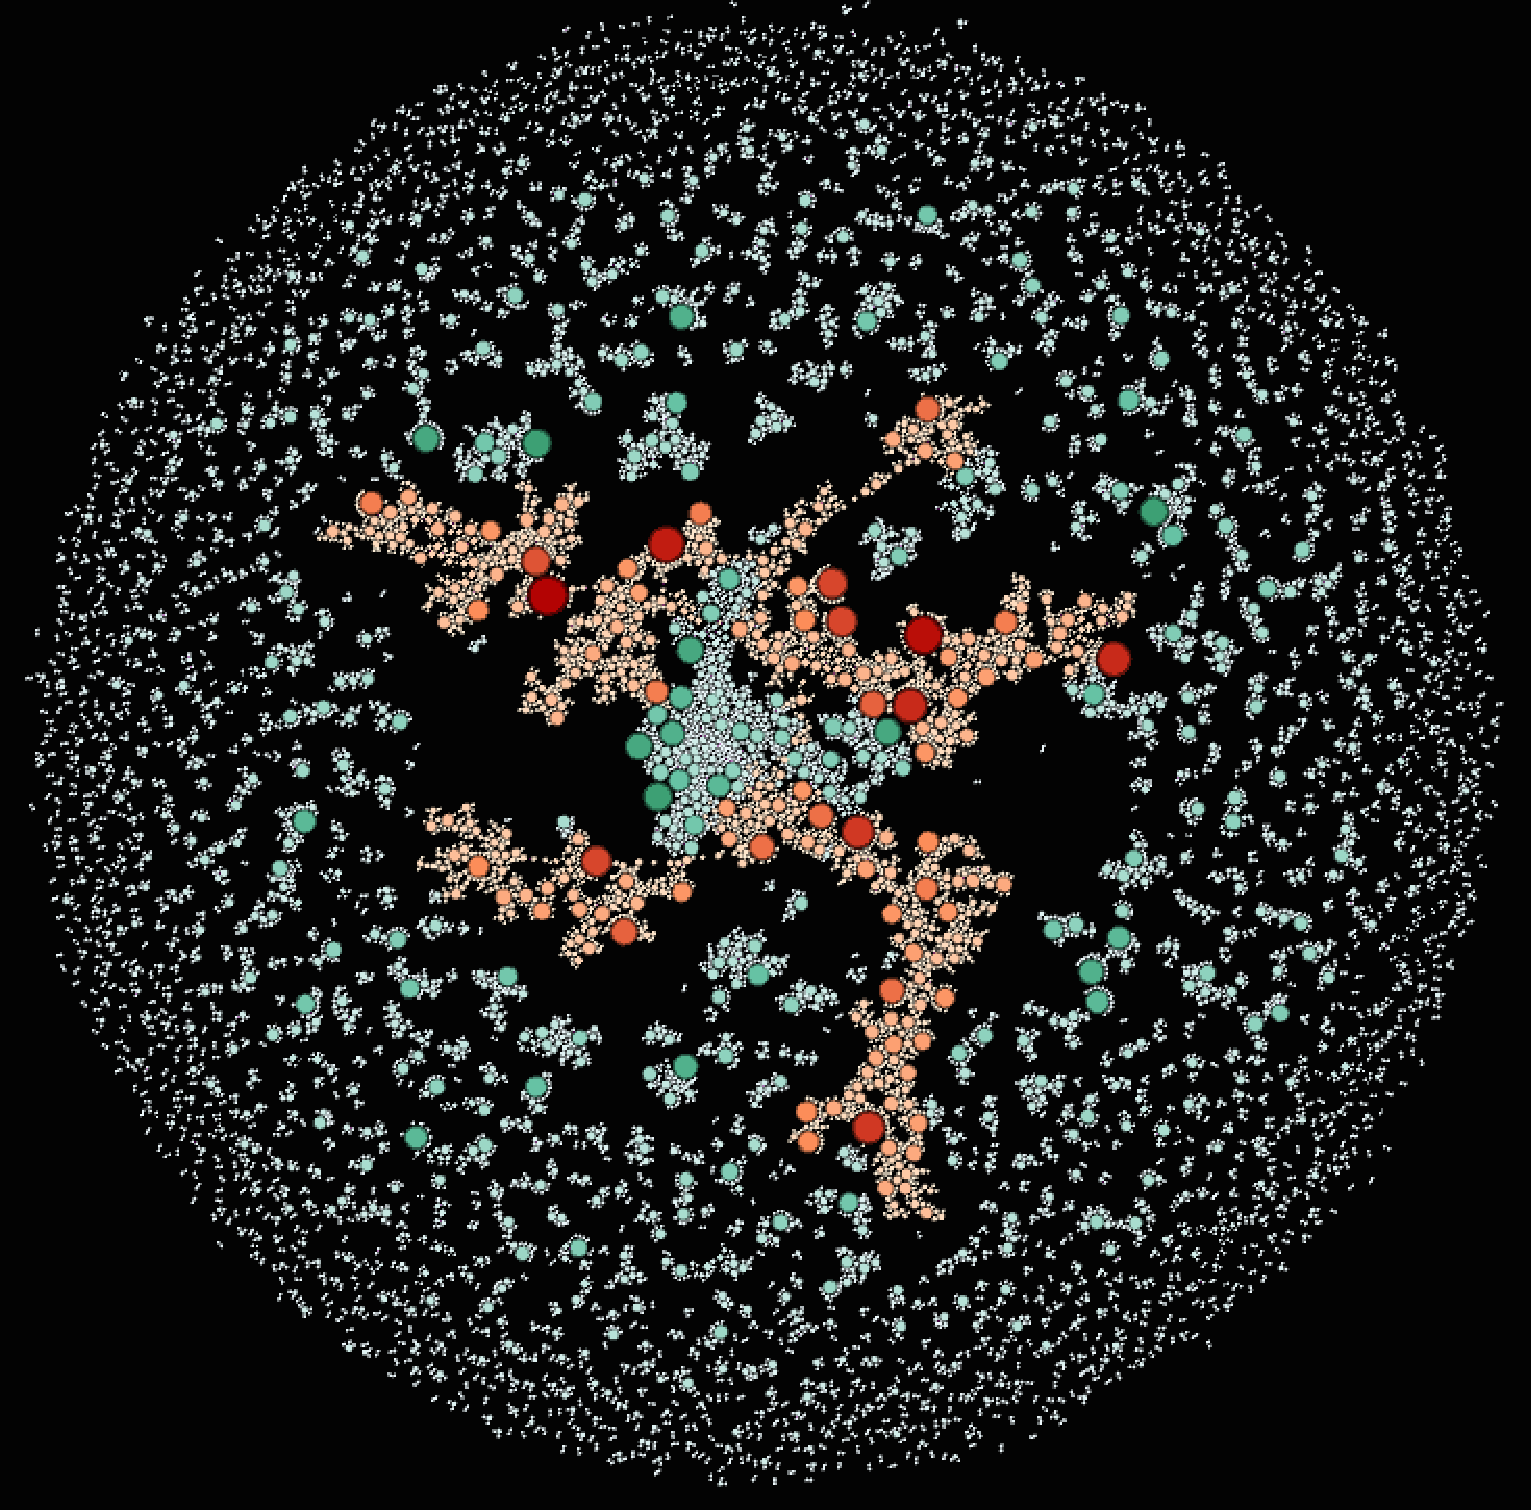
\includegraphics[width = 0.3\textwidth]{ProgramsImages/sexualNetworkNOLA}
\end{center}
\caption{Heterosexual network for the stochastic simulations of STD transmission.}
\label{netmodel}
\end{wrapfigure}\Upara{Stochastic Network Model for Spread of Sexually Transmitted Diseases} The previous climate models are deterministic models, where multiple simulates with the same parameter values predict identical results. 
For the past six years, MH has been collaborating with the Tulane School of 
Public Health and Tropical Medicine to develop a stochastic Monte Carlo Markov Chain agent-based model for the transmission of sexually transmitted diseases (STDs) in New Orleans \cite{azizi2016multi,azizi2018using,chowell2016mathematical}. 
The STIs spread through a dynamic heterosexual bipartite network of up to 200,000 nodes and includes treatment, contact tracing, condom use, and partner notification. The network changes each day as people change their short-term and long-term partnerships. 
Since the partnership network and disease transmission is modeled as a stochastic process, multiple simulations with the same parameter values produce a multivariate distribution of QOIs. Each ensemble of runs can take hours on the Tulane Cypress 300+ TFlop supercomputer. 
\emph{We will use our adaptive sampling to optimize the simulations comparing mitigation strategies for slowing the spread of STIs.} 
The mean-field MLS model will identify the underlying trends in the predictions, and the kriging Gaussian Process model will quantify the aleatory uncertainty created by the stochastic events.


%%%%%%%%%%%%%%%%%%%%%%%%%%%%%%%%%%%%%%%%%%%%%%%%%%%%%%%%%%%%%%%%%%%%%%%%%%%%%%%%%%%
\subsection{Software} \label{sec:Software}
%%%%%%%%%%%%%%%%%%%%%%%%%%%%%%%%%%%%%%%%%%%%%%%%%%%%%%%%%%%%%%%%%%%%%%%%%%%%%%%%%%%
There is considerable interest in computational mathematics, computer science, and engineering communities in developing and using software for the adaptive design and analysis of computer experiments. Examples of existing packages are the MATLAB libraries UQLab \cite{UQLab2014}, SUMO\cite{SUMO2010}, ooDACE \cite{ooDACE2014} (a successor to DACE \cite{dace2002}), and CODES \cite{CODES2015}, and the Python libraries emukit \cite{emukit2019}, SMT \cite{SMT2019}, and pySOT \cite{pySOT2015}. Many of these packages employ allow for trends and variation modeling via kriging, but not they are not as flexible as those we intend to develop.

Our algorithms will be implemented in libraries on open source repositories for use by the modeling community. We will compare the performance of our algorithms with existing software using test cases in the literature and on the large applications described above. We will also explore collaborations with the developers of software libraries whose interests overlap ours so that we can leverage each others' strengths.

%%%%%%%%%%%%%%%%%%%%%%%%%%%%%%%%%%%%%%%%%%%%%%%%%%%%%%%%%%%%%%%%%%%%%%%%%%%%%%%%%%%

\section{Broader Impacts}

%%%%%%%%%%%%%%%%%%%%%%%%%%%%%%%%%%%%%%%%%%%%%%%%%%%%%%%%%%%%%%%%%%%%%%%%%%%%%%%%%%%
The PIs will collaborate with junior scholars, including students at the high school through PhD level. Because this project spans theory, algorithms, applications, and software, we will be able to mentor our junior scholars in the areas that they have particular interest or ability, while helping them to understand the spectrum of expertise required to solve these kinds of problems. The PIs will also engage in giving tutorials and teaching courses that will include our new results.

%%%%%%%%%%%%%%%%%%%%%%%%%%%%%%%%%%%%%%%%%%%%%%%%%%%%
\Upara{Mentoring}
%%%%%%%%%%%%%%%%%%%%%%%%%%%%%%%%%%%%%%%%%%%%%%%%%%%%
\FH and MH lead regular research group meetings at their respective institutions comprised of long-term and short-term student collaborators, visitors, the curious, and special guests. Ongoing work in early or polished stages is shared. Papers of other authors are presented. Mentoring takes place during these meetings, as well as individually.

%%%%%%%%%%%%%%%%%%%%%%%%%%%%%%%%%%%%%%%%%%%%%%%%%%%%
\begin{sloppypar}\Upara{Providing Research Experiences for Undergraduate and High School Students} 
%%%%%%%%%%%%%%%%%%%%%%%%%%%%%%%%%%%%%%%%%%%%%%%%%%%%
Our project will support two summer undergraduate students per year at Illinois Tech, or possibly at LANL. As in the past, the NSF funds will be a catalyst for seeking additional funds to support summer students. In choosing summer students, we will make a deliberate effort to diverse research environment by targeting female and underrepresented minority students as well as students from less research-focused institutions (see Sect.~\ref{prevBIsect}). We will also welcome well-prepared high school students to join our research group.\end{sloppypar}

%%%%%%%%%%%%%%%%%%%%%%%%%%%%%%%%%%%%%%%%%%%%%%%%%%%%
\Upara{Preparing Students for Academic Careers} 
%%%%%%%%%%%%%%%%%%%%%%%%%%%%%%%%%%%%%%%%%%%%%%%%%%%%
Mentoring is a multi-faceted and 
potentially long-term process continuing even after the mentee has moved on from Illinois Tech. 
Our PhD students gain experience in both research and mentoring the younger students in our research group. We 
continue contact with many of our former students, in particular Yiou Li (female). We will continue to help our students prepare for academic careers and continue mentoring them after they leave Illinois Tech.

%%%%%%%%%%%%%%%%%%%%%%%%%%%%%%%%%%%%%%%%%%%%%%%%%%%%
\Upara{Preparing Students for Industry Careers}
%%%%%%%%%%%%%%%%%%%%%%%%%%%%%%%%%%%%%%%%%%%%%%%%%%%%
We also help current students land 
competitive jobs in the business world. Our training in the areas of computation and software 
development gives our students the needed edge in comparison to other mathematics 
graduates. For example, LlAJR and XZ are working in the financial services industry and LJ is 
working in marketing analytics. All of them are developing and testing quantitatively sophisticated and computationally intensive models. 

%%%%%%%%%%%%%%%%%%%%%%%%%%%%%%%%%%%%%%%%%%%%%%%%%%%%
\Upara{Giving Tutorials and Invited Lectures}
%%%%%%%%%%%%%%%%%%%%%%%%%%%%%%%%%%%%%%%%%%%%%%%%%%%%
We will continue providing lectures to students at various stages in their careers, ranging from high school to graduate school. These encourage students to enter STEM and encourage STEM students 
to engage in research in general and this research area in particular.


%%%%%%%%%%%%%%%%%%%%%%%%%%%%%%%%%%%%%%%%%%%%%%%%%%%%
%\subsection{Contributions to Resources in Research, Education and the Broader Society} 
%\label{BroaderTwoSec}
%%%%%%%%%%%%%%%%%%%%%%%%%%%%%%%%%%%%%%%%%%%%%%%%%%%%

\Upara{Crossing Disciplinary Boundaries} The proposed research straddles mathematics, statistics, theoretical computer science, and 
application areas. The PIs have complementary strengths that facilitate this interdisciplinary research. YD has expertise in adaptive algorithms and software development. \FH has expertise in adaptive algorithms, low discrepancy sampling, kernel-based methods, and tractability. MH has expertise in modeling of large scale phenomena and algorithm development. Our expertise provides both an obligation and an opportunity to interact with a number of diverse communities.

%%%%%%%%%%%%%%%%%%%%%%%%%%%%%%%%%%%%%%%%%%%%%%%%%%%%
\Upara{Disseminating Research and Writing Survey Papers}
%%%%%%%%%%%%%%%%%%%%%%%%%%%%%%%%%%%%%%%%%%%%%%%%%%%%
The research supported by this grant will result in publications in peer-reviewed journals in applied mathematics, computer science, statistics, and science/engineering. These 
journals will include both those that emphasize theory and those that emphasize applications. The PIs will continue their practice of writing tutorial, survey, and encyclopedia articles. These will make our findings accessible to a wider audience.


%%%%%%%%%%%%%%%%%%%%%%%%%%%%%%%%%%%%%%%%%%%%%%%%%%%%
\Upara{Organizing and Presenting at Conferences}
%%%%%%%%%%%%%%%%%%%%%%%%%%%%%%%%%%%%%%%%%%%%%%%%%%%%
Our students and postdocs involved in this project will join us in presenting our results at conferences and workshops. These include: (i) specialized meetings focusing on approximation theory, complexity, 
experimental design, Monte Carlo methods, and probabilistic numerics; (ii) the national meetings of AMS, SIAM, and the statistical societies; and (iii) conferences devoted to application areas. We are frequently invited to speak at such conferences, which will give our results a prominent hearing. We will also continue to organize specialized conferences or minisymposia within larger conferences.

%%%%%%%%%%%%%%%%%%%%%%%%%%%%%%%%%%%%%%%%%%%%%%%%%%%%
\Upara{Bridging Applied Mathematics and Statistics}
%%%%%%%%%%%%%%%%%%%%%%%%%%%%%%%%%%%%%%%%%%%%%%%%%%%%
This project touches on topics that are of interest to the statistics community: kriging, Monte Carlo methods, probabilistic numerics, and design of experiments. We have and will continue to engage the statistics community 
by speaking their conferences and departmental colloquia.

%%%%%%%%%%%%%%%%%%%%%%%%%%%%%%%%%%%%%%%%%%%%%%%%%%%%
\Upara{Establishing a New Paradigm for Adaptive Algorithms} 
%%%%%%%%%%%%%%%%%%%%%%%%%%%%%%%%%%%%%%%%%%%%%%%%%%%%
The idea of adaptive algorithms where the sampling scheme and the norm of the input function adapt to the output data is uncommon in the computational mathematics literature. The derivation of theory for adaptive algorithms based on cones is also new. These ideas have potential applications to other numerical problems beyond those studied in the proposed research. We will continue to promote these ideas among numerical analysts and computational complexity theorists. The recent work by Kunsch, Novak, and Rudolf \cite{KunEtal19a} shows that the idea of cones is catching on.

%%%%%%%%%%%%%%%%%%%%%%%%%%%%%%%%%%%%%%%%%%%%%%%%%%%%
\begin{sloppypar}\Upara{Creating Software and Collaborating with Software Developers}
%%%%%%%%%%%%%%%%%%%%%%%%%%%%%%%%%%%%%%%%%%%%%%%%%%%%
Our algorithms will be implemented in freely available software on public repositories. We will discuss with software developers whose packages have complementary capabilities how we might collaborate. We expect our new algorithms to be incorporated into widely used numerical packages, as was done for our algorithm in \cite{HonHic00a} by \MATLAB and \NAG. The \MATLAB \GAIL library \citep{ChoEtal19a}, developed by \FH, \YD, and collaborators, contains univariate function approximation and minimization algorithms, as well as multivariate integration algorithms. A project to a community-based quasi-Monte Carlo Python library QMCPy, is underway with corporate sponsorship. \end{sloppypar}

%%%%%%%%%%%%%%%%%%%%%%%%%%%%%%%%%%%%%%%%%%%%%%%%%%%%
\section{Project Management and Collaboration}
%%%%%%%%%%%%%%%%%%%%%%%%%%%%%%%%%%%%%%%%%%%%%%%%%%%%
This research will be primarily conducted at Illinois Tech, Tulane U, and Los Alamos National Laboratory (LANL), where MH has a visiting scientist appointment. \FH will lead the effort at Illinois Tech, and MH will lead the effort at Tulane. \FH and \YD will focus on the theoretical analysis of the algorithms, including error bounds for the surrogate models. They will also lead the exploration of the data-inferred reproducing/covariance kernels. MH will focus on the design of our novel algorithms, including the weighted least squares and the Bayesian bootstrap. He will also lead the application of our new algorithms to the large-scale application problems. 

The PhD student will be based at Illinois Tech during the academic year under the direct supervision of \FH and \YD. The PhD student will collaborate with us on algorithmic developments, its theoretical analysis, and its implementation in freely available software. During the summer, the PhD student will join MH in Los Alamos and be involved with testing our algorithms on challenging application problems. The undergraduate students will work either at Illinois Tech or at LANL during the summer exploring interesting, bite-sized aspects of the algorithms and their performance.

Our research groups will meet regularly via video conference and in person a couple of times per year at one of our campuses or at conferences.

\section{Results from Prior NSF Support} \label{sec:prior_work}

\subsection{NSF-DMS-1522687\except{toc}{, \emph{Stable, Efficient, Adaptive Algorithms for
			Approximation and Integration},
		\$270,000, August 2015 -- July 2018}
} \label{sec:PreviousFred}
%%%%%%%%%%%%%%%%%%%%%%%%%%%%%%%%%%%%%%%%%%%%%%%%%%%%%%%%%%%%%%%%%%%%%%%%%%%%%%%%%%%

\hypertarget{GEFlink}{Gregory E.\ Fasshauer} (\GEF, co-PI) and \FH (PI) led this project, along with  \hypertarget{SCTClink}{Sou-Cheng Terrya Choi} (\SCTC, Senior Personnel).  Other major contributors were \FH's research students  \YD (PhD 2015), \hypertarget{LlAJRlink}{Llu\'is Antoni Jim\'enez Rugama} (\LJ, 2016),
\LlAJR (PhD 2016), \hypertarget{DLlink}{Da Li} (\DL, MS 2016), \hypertarget{JLlink}{Jiazhen Liu} (\JL, MS 2018), JR (PhD 2019), \hypertarget{XTlink}{Xin Tong} (\XT, MS 2014, PhD 2020 @ University of Illinois at Chicago), \hypertarget{KZlink}{Kan Zhang} \KZ, PhD student), \hypertarget{YZlink}{Yizhi Zhang} (\YZ, PhD 2018), and \hypertarget{XZlink}{Xuan Zhou} (\XZ, PhD 2015).  Articles, theses,
software, and preprints supported in
part by this
grant
include
\cite{ala_augmented_2017,
	ChoEtal17a,
	ChoEtal20a,
	Din15a,
	DinHic20a,
	GilEtal16a,
	Hic17a,
	HicJag18b,
	HicJim16a,
	HicEtal18a,
	HicEtal17a,
	HicKriWoz19a,
	RatHic19a,
	GilJim16b,
	JimHic16a,
	JohFasHic18a,
	Li16a,
	Liu17a,
	MarEtal18a,
	mccourt_stable_2017,
	MCCEtal19a,
	mishra_hybrid_2018,
	MisEtal19a,
	rashidinia_stable_2016,
	rashidinia_stable_2018,
	Zha18a,
	Zha17a,
	Zho15a,
	ZhoHic15a}.

%%%%%%%%%%%%%%%%%%%%%%%%%%%%%%%%%%%%%%%%%%%%%%%%%%%%%%%%%%%%%%%%%%%%%%%%%%%%%%%%%%%
\subsubsection{Intellectual Merit from Prior NSF Support}
\label{previousmeritsubsec}
%%%%%%%%%%%%%%%%%%%%%%%%%%%%%%%%%%%%%%%%%%%%%%%%%%%%%%%%%%%%%%%%%%%%%%%%%%%%%%%%%%%
\phantom{a}

\iffalse
\begin{wrapfigure}{r}{0.4\textwidth}
	\centering
	\vspace{-1ex}
	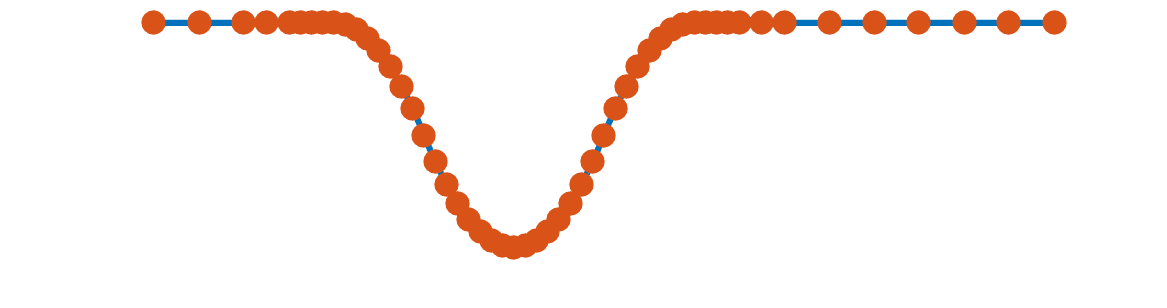
\includegraphics[width = 0.4\textwidth]{ProgramsImages/sampling-funappxg.png}
	\\
	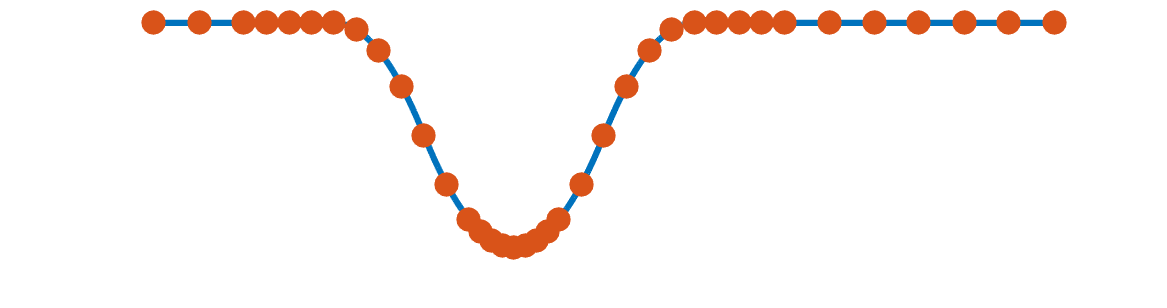
\includegraphics[width = 0.4\textwidth]{ProgramsImages/sampling-funming.png}
	
	\vspace{-2ex}
	\caption{The function data ({\color{MATLABOrange}$\bullet$}) for the locally adaptive
		function approximation (top) and minimization (bottom) algorithms in \cite{ChoEtal17a}.  Sampling is denser where $\abs{f''}$ is larger.  For minimization it is also denser where the function values are smaller. \label{localadaptfig}}
\end{wrapfigure}
\fi

\Upara{Adaptive Algorithms for Univariate Problems}
\FH, \SCTC, \YD, \XT, \YZ and collaborators developed adaptive algorithms for univariate integration, function approximation, and optimization \cite{ChoEtal17a,HicEtal14b,  Din15a, Ton14a, Zha18a}.  The in \cite{ChoEtal17a} are \emph{locally adaptive}---the nonuniform sampling density is influenced by the function data.  For function approximation, the computational cost to achieve an error tolerance of $\varepsilon$ is $\Order\left(\sqrt{\norm[1/2]{f''}/\varepsilon} \right)$, which is essentially optimal.  The $1/2$-quasinorm $\norm[1/2]{f''}$ may be much smaller than
$\norm[\infty]{f''}$ for peaky functions.


\Upara{Globally Adaptive Cubature Based on Low Discrepancy (LD) Sequences}
\FH, \LlAJR, \DL, and \JR developed globally adaptive algorithms for approximating $\int_{[0,1]^d} f(\bx) \, \dif \bx$ based on LD sequences \cite{HicJim16a,HicEtal17a,JimHic16a,RatHic19a}.  The error bounds underlying these adaptive cubatures rely on the Fourier coefficients of the sampled function values, either by tracking their decay rate or by using them to construct Bayesian credible intervals.  In the latter case, choosing covariance kernels that match the LD sequences reduces the computational cost to $\Order(n \log(n))$, making Bayesian cubature practical.

\Upara{Multivariate Function Approximation}
\FH, \YD, and \LlAJR and collaborators investigated function approximation problems for Banach spaces, $\calf$, defined by series representations \cite{DinHic20a,DinEtal20a}.  Again cones, $\calc \subset \calf$, of reasonable candidate functions were defined.  Adaptive function approximation algorithms constructed were shown to be essentially optimal.


%%%%%%%%%%%%%%%%%%%%%%%%%%%%%%%%%%%%%%%%%%%%%%%%%%%%%%%%%%%%%%%%%%%%%%%%%%%%%%%%%%%
\subsubsection{Broader Impacts from Prior NSF Support} \label{prevBIsect}
%%%%%%%%%%%%%%%%%%%%%%%%%%%%%%%%%%%%%%%%%%%%%%%%%%%%%%%%%%%%%%%%%%%%%%%%%%%%%%%%%%%
\phantom{a}

\Upara{Publications, Conference Participation, Conference Organization, and Leadership} Publications by \GEF, \FH,  \SCTC, students, and collaborators are listed above.  The project personnel spoke at many academic conferences and gave colloquium/seminar talks to mathematics and
statistics departments.  \FH co-organized the
2016 Spring Research
Conference.   \FH gave an invited tutorial
at MCQMC 2016
\cite{Hic17a}, a biennial conference for which he serves on the steering committee.  \FH
was a program leader for the SAMSI 2017--18 Quasi-Monte Carlo (QMC) Program.   \FH received the 2016 Joseph F.\ Traub Prize for Achievement in Information-Based Complexity.  \FH was appointed the director of Illinois Tech's new Center for Interdisciplinary
Scientific Computation in 2017.  In 2018, \FH was appointed Vice Provost for Research.

\Upara{\GAIL Software} The algorithms from this research have been implemented in
\GAIL, our open source \MATLAB library hosted on
Github with input parsing, input validation, unit tests, inline documentation, and
demonstrations. \SCTC has been key in this effort.  \GAIL has been used in the yearly graduate course in Monte Carlo methods taught by \FH and \YD.
%With the help of students, we are starting to port GAIL to Python and \Rlang.

\Upara{Boosting the STEM Workforce} \GEF, \FH, and \SCTC mentored a number of
research students associated with this project.  Female students include \YD, \LJ, \JL, \XT, and Xiaoyang Zhao (MS 2017).   Mentees include more than a dozen
Brazilian Science Mobility Program students in the summers of 2015 and 2016, plus eight other students (two female) from Illinois Tech, Biola U, U Minnesota, Macalester U, NUS, Colorado School of Mines.  Seven of these eight have enrolled in graduate programs.  


\subsection{Prior NSF Support James M Hyman} \label{sec:prior}
\vspace{0.1cm}
Dr. James M. Hyman was the PI for the NSF/NIH project (1563531) on \textit{Multiscale Models for Predicting the Effectiveness of Mitigation Efforts in Controlling Vector-Borne Epidemics}, Awarded Amount: \$434,289.00,  period of support: 05/01/2016-04/30/2019.  
We created and analyzed a new class of mathematical models to forecast the spread of emerging mosquito-borne diseases.  The new model included behavior change in the human population and the impact of infecting wild mosquitoes with Wolbachia in mitigating these diseases. 
\textit{ Broader Impact:}   We mentored several undergraduate capstone projects, honor's thesis and graduate Master's dissertations and two PhD dissertations in mathematics and at the Tulane School for Public Health and Tropical Medicine on the modeling of mosquito-borne diseases. 
\textit{ Publications:} \cite{xue2016two,xue2018comparing,qu2018modeling,moran2016epidemic,chowell2016mathematical,margevicius2016biosurveillance}

\newpage
\clearpage
%\pagenumbering{arabic}
\setcounter{page}{1}
%\renewcommand{\thepage}{D-\arabic{page}}

\bibliographystyle{spbasic.bst}


{\renewcommand\addcontentsline[3]{} 
\renewcommand{\refname}{{\Large\textbf{References Cited}}} %%
\renewcommand{\bibliofont}{\normalsize}

\bibliography{DoE_MH,FJH23,FJHown23,yuhan}}
\end{document}
